\section{Camera Calibration and 3D Reconstruction}

The functions in this section use the so-called pinhole camera model. That
is, a scene view is formed by projecting 3D points into the image plane
using a perspective transformation.

\[
s \; m' = A [R|t] M'
\]

or

\[
s \vecthree{u}{v}{1} = \vecthreethree
{fx}{0}{cx}
{0}{fy}{cy}
{0}{0}{1}
\begin{bmatrix}
 r_{11} & r_{12} & r{13} & t_1 \\
 r_{21} & r_{22} & r{23} & t_2 \\
 r_{31} & r_{32} & r{33} & t_3
\end{bmatrix}
\begin{bmatrix}X\\Y\\Z\\1 \end{bmatrix}
\]

Where $(X, Y, Z)$ are the coordinates of a 3D point in the world
coordinate space, $(u, v)$ are the coordinates of the projection point
in pixels. $A$ is called a camera matrix, or a matrix of
intrinsic parameters. $(cx, cy)$ is a principal point (that is
usually at the image center), and $fx, fy$ are the focal lengths
expressed in pixel-related units. Thus, if an image from camera is
scaled by some factor, all of these parameters should
be scaled (multiplied/divided, respectively) by the same factor. The
matrix of intrinsic parameters does not depend on the scene viewed and,
once estimated, can be re-used (as long as the focal length is fixed (in
case of zoom lens)). The joint rotation-translation matrix $[R|t]$
is called a matrix of extrinsic parameters. It is used to describe the
camera motion around a static scene, or vice versa, rigid motion of an
object in front of still camera. That is, $[R|t]$ translates
coordinates of a point $(X, Y, Z)$ to some coordinate system,
fixed with respect to the camera. The transformation above is equivalent
to the following (when $z \ne 0$):

\[
\begin{array}{l}
\vecthree{x}{y}{z} = R \vecthree{X}{Y}{Z} + t\\
x' = x/z\\
y' = y/z\\
u = f_x*x' + c_x\\
v = f_y*y' + c_y
\end{array}
\]

Real lenses usually have some distortion, mostly
radial distorion and slight tangential distortion. So, the above model
is extended as:

\[
\begin{array}{l}
\vecthree{x}{y}{z} = R \vecthree{X}{Y}{Z} + t\\
x' = x/z\\
y' = y/z\\
x'' = x' (1 + k_1 r^2 + k_2 r^4 + k_3 r^6) + 2 p_1 x' y' + p_2(r^2 + 2 x'^2) \\
y'' = y' (1 + k_1 r^2 + k_2 r^4 + k_3 r^6) + p_1 (r^2 + 2 y'^2) + 2 p_2 x' y' \\
\text{where} \quad r^2 = x'^2 + y'^2 \\
u = f_x*x'' + c_x\\
v = f_y*y'' + c_y
\end{array}
\]

$k_1$, $k_2$, $k_3$ are radial distortion coefficients, $p_1$, $p_2$ are tangential distortion coefficients.
Higher-order coefficients are not considered in OpenCV.
The distortion coefficients do not depend on the scene viewed, thus they also belong to the intrinsic camera parameters.
\emph{And they remain the same regardless of the captured image resolution.}
That is, if, for example, a camera has been calibrated on images of $320
\times 240$ resolution, absolutely the same distortion coefficients can
be used for images of $640 \times 480$ resolution from the same camera (while $f_x$,
$f_y$, $c_x$ and $c_y$ need to be scaled appropriately).

The functions below use the above model to

\begin{itemize}
 \item Project 3D points to the image plane given intrinsic and extrinsic parameters
 \item Compute extrinsic parameters given intrinsic parameters, a few 3D points and their projections.
 \item Estimate intrinsic and extrinsic camera parameters from several views of a known calibration pattern (i.e. every view is described by several 3D-2D point correspodences).
\end{itemize}

\ifCPy

\cvCPyFunc{CalcImageHomography}
Calculates the homography matrix for an oblong planar object (e.g. arm).

\cvcodeC{
void cvCalcImageHomography( \par float* line,\par CvPoint3D32f* center,\par float* intrinsic,\par float* homography );
}\cvcodePy{CalcImageHomography(line,points)-> intrinsic,homography}

\begin{description}
\cvarg{line}{the main object axis direction (vector (dx,dy,dz))}
\cvarg{center}{object center ((cx,cy,cz))}
\cvarg{intrinsic}{intrinsic camera parameters (3x3 matrix)}
\cvarg{homography}{output homography matrix (3x3)}
\end{description}

The function calculates the homography
matrix for the initial image transformation from image plane to the
plane, defined by a 3D oblong object line (See \_\_Figure 6-10\_\_
in the OpenCV Guide 3D Reconstruction Chapter).


\cvCPyFunc{CalibrateCamera2}
Finds the intrinsic and extrinsic camera parameters using a calibration pattern.

\cvcodeC{
void cvCalibrateCamera2( \par const CvMat* object\_points,\par const CvMat* image\_points,\par const CvMat* point\_counts,\par CvSize image\_size,\par CvMat* intrinsic\_matrix,\par CvMat* distortion\_coeffs,\par CvMat* rotation\_vectors=NULL,\par CvMat* translation\_vectors=NULL,\par int flags=0 );
}\cvcodePy{CalibrateCamera2(object\_points,image\_points,point\_counts,image\_size,intrinsic\_matrix,distortion\_coeffs,rotation\_vectors,translation\_vectors,flags=0)-> None}

\begin{description}
\cvarg{object\_points}{The joint matrix of object points, 3xN or Nx3, where N is the total number of points in all views}
\cvarg{image\_points}{The joint matrix of corresponding image points, 2xN or Nx2, where N is the total number of points in all views}
\cvarg{point\_counts}{Vector containing the number of points in each particular view, 1xM or Mx1, where M is the number of points in a scene}
\cvarg{image\_size}{Size of the image, used only to initialize the intrinsic camera matrix}
\cvarg{intrinsic\_matrix}{The output camera matrix $A = \vecthreethree{fx}{0}{cx}{0}{fy}{cy}{0}{0}{1} $. If \texttt{CV\_CALIB\_USE\_INTRINSIC\_GUESS} and/or \texttt{CV\_CALIB\_FIX\_ASPECT\_RATION} are specified, some or all of \texttt{fx, fy, cx, cy} must be initialized}
\cvarg{distortion\_coeffs}{The output 4x1 or 1x4 vector of distortion coefficients $k_1, k_2, k_3, k_4$}
\cvarg{rotation\_vectors}{The output 3xM or Mx3 array of rotation vectors (compact representation of rotation matrices, \cvCPyCross{Rodrigues2})}
\cvarg{translation\_vectors}{The output 3xM or Mx3 array of translation vectors}
\cvarg{flags}{Different flags, may be 0 or combination of the following values:
\begin{description}
\cvarg{CV\_CALIB\_USE\_INTRINSIC\_GUESS}{\texttt{intrinsic\_matrix} contains the valid initial values of \texttt{fx, fy, cx, cy} that are optimized further. Otherwise, \texttt{(cx, cy)} is initially set to the image center (\texttt{image\_size} is used here), and focal distances are computed in some least-squares fashion. Note, that if intrinsic parameters are known, there is no need to use this function. Use \cvCPyCross{FindExtrinsicCameraParams2} instead.}
\cvarg{CV\_CALIB\_FIX\_PRINCIPAL\_POINT}{The principal point is not changed during the global optimization, it stays at the center and at the other location specified (when \texttt{CV\_CALIB\_USE\_INTRINSIC\_GUESS} is set as well)}
\cvarg{CV\_CALIB\_FIX\_ASPECT\_RATIO}{The optimization procedure considers only one of \texttt{fx} and \texttt{fy} as independent variables and keeps the aspect ratio \texttt{fx/fy} the same as it was set initially in \texttt{intrinsic\_matrix}. In this case the actual initial values of \texttt{(fx, fy)} are either taken from the matrix (when \texttt{CV\_CALIB\_USE\_INTRINSIC\_GUESS} is set) or estimated somehow (in the latter case \texttt{fx, fy} may be set to arbitrary values, only their ratio is used).}
\cvarg{CV\_CALIB\_ZERO\_TANGENT\_DIST}{Tangential distortion coefficients are set to zeros and do not change during the optimization.}}
\end{description}
\end{description}

The function estimates the intrinsic camera
parameters and extrinsic parameters for each of the views. The
coordinates of 3D object points and their correspondent 2D projections
in each view must be specified. That may be achieved by using an
object with known geometry and easily detectable feature points.
Such an object is called a calibration rig or calibration pattern,
and OpenCV has built-in support for a chessboard as a calibration
rig (see \cvCPyCross{FindChessboardCornerGuesses}). Currently, initialization
of intrinsic parameters (when \texttt{CV\_CALIB\_USE\_INTRINSIC\_GUESS}
is not set) is only implemented for planar calibration rigs
(z-coordinates of object points must be all 0's or all 1's). 3D
rigs can still be used as long as initial \texttt{intrinsic\_matrix}
is provided. After the initial values of intrinsic and extrinsic
parameters are computed, they are optimized to minimize the total
back-projection error - the sum of squared differences between the
actual coordinates of image points and the ones computed using
\cvCPyCross{ProjectPoints2}.

Note: if you're using a non-square (=non-NxN) grid and
\cvCPyCross{FindChessboardCorners} for calibration, and cvCalibrateCamera2 returns
bad values (i.e. zero distortion coefficients, an image center of
(w/2-0.5,h/2-0.5), and / or large differences between $fx$ and $fy$ (ratios of
10:1 or more)), then you've probaby  used pattern\_size=cvSize(rows,cols),
but should use pattern\_size=cvSize(cols,rows) in \cvCPyCross{FindChessboardCorners}.

\cvCPyFunc{ComputeCorrespondEpilines}
For points in one image of a stereo pair, computes the corresponding epilines in the other image.

\cvcodeC{
void cvComputeCorrespondEpilines( \par const CvMat* points,\par int which\_image,\par const CvMat* fundamental\_matrix,\par CvMat* correspondent\_lines);
}\cvcodePy{ComputeCorrespondEpilines(points, which\_image, fundamental\_matrix, correspondent\_lines) -> None}

\begin{description}
\cvarg{points}{The input points. \texttt{2xN, Nx2, 3xN} or \texttt{Nx3} array (where \texttt{N} number of points). Multi-channel \texttt{1xN} or \texttt{Nx1} array is also acceptable}
\cvarg{which\_image}{Index of the image (1 or 2) that contains the \texttt{points}}
\cvarg{fundamental\_matrix}{Fundamental matrix}
\cvarg{correspondent\_lines}{Computed epilines, a \texttt{3xN} or \texttt{Nx3} array}
\end{description}

For every point in one of the two images of a stereo-pair the function
\texttt{ComputeCorrespondEpilines} finds the equation of a line that
contains the corresponding point (i.e. projection of the same 3D
point) in the other image. Each line is encoded by a vector of 3
elements $l = \vecthree{a}{b}{c}$ so that:

\[ l^T \vecthree{x}{y}{1} = 0 \]
or
\[ a x + b y + c = 0 \]

From the fundamental matrix definition (see \cvCPyCross{FindFundamentalMatrix}
discussion), line $l_1$ for a point $p_1$ in the first image
$(\texttt{which\_image} =1)$ can be computed as:

\[ l_2 = F p_1 \]

and the line $l_1$ for a point $p_2$ in the second image $(\texttt{which\_image} =1)$ can be computed as:

\[ l_1 = F^T p_2 \]

Line coefficients are defined up to a scale. They are normalized $(a^2+b^2=1)$ are stored into \texttt{correspondent\_lines}.

\cvCPyFunc{ConvertPointsHomogenious}
Convert points to/from homogenious coordinates.

\cvcodeC{
void cvConvertPointsHomogenious( \par const CvMat* src,\par CvMat* dst );
}

\begin{description}
\cvarg{src}{The input point array, \texttt{2xN, Nx2, 3xN, Nx3, 4xN or Nx4 (where \texttt{N} is the number of points)}. Multi-channel \texttt{1xN} or \texttt{Nx1} array is also acceptable}
\cvarg{dst}{The output point array, must contain the same number of points as the input; The dimensionality must be the same, 1 less or 1 more than the input, and also within 2 to 4}
\end{description}

The function converts 2D or 3D points from/to homogenious coordinates, or simply copies or transposes the array. If the input array dimensionality is larger than the output, each coordinate is divided by the last coordinate:

\[
\begin{array}{l}
(x,y[,z],w) -> (x',y'[,z'])\\
\text{where} \\
x' = x/w \\
y' = y/w \\
z' = z/w \quad \text{(if output is 3D)}
\end{array}
\]

If the output array dimensionality is larger, an extra 1 is appended to each point.  Otherwise, the input array is simply copied (with optional tranposition) to the output.

\textbf{Note} because the function accepts a large variety of array layouts, it may report an error when input/output array dimensionality is ambiguous. It is always safe to use the function with number of points $\texttt{N} \ge 5$, or to use multi-channel \texttt{Nx1} or \texttt{1xN} arrays.

\cvCPyFunc{CreatePOSITObject}
Initializes a structure containing object information.

\cvcodeC{
CvPOSITObject* cvCreatePOSITObject( \par CvPoint3D32f* points,\par int point\_count );
}\cvcodePy{CreatePOSITObject(points)-> POSITObject}

\begin{description}
\cvarg{points}{Pointer to the points of the 3D object model}
\cvarg{point\_count}{Number of object points}
\end{description}

The function allocates memory for the object structure and computes the object inverse matrix.

The preprocessed object data is stored in the structure \cvCPyCross{CvPOSITObject}, internal for OpenCV, which means that the user cannot directly access the structure data. The user may only create this structure and pass its pointer to the function.

An object is defined as a set of points given in a coordinate system. The function \cvCPyCross{POSIT} computes a vector that begins at a camera-related coordinate system center and ends at the \texttt{points[0]} of the object.

Once the work with a given object is finished, the function \cvCPyCross{ReleasePOSITObject} must be called to free memory.

\cvCPyFunc{CreateStereoBMState}
Creates block matching stereo correspondence structure.

\begin{lstlisting}
#define CV_STEREO_BM_BASIC 0
#define CV_STEREO_BM_FISH_EYE 1
#define CV_STEREO_BM_NARROW 2
\end{lstlisting}

\cvcodeC{

CvStereoBMState* cvCreateStereoBMState( int preset=CV\_STEREO\_BM\_BASIC,
                                        int numberOfDisparities=0 );

}\cvcodePy{CreateStereoBMState(preset=CV\_STEREO\_BM\_BASIC,numberOfDisparities=0)-> StereoBMState}

\begin{description}
\cvarg{preset}{ID of one of the pre-defined parameter sets. Any of the parameters can be overridden after creating the structure.}
\cvarg{numberOfDisparities}{The number of disparities. If the parameter is 0, it is taken from the preset, otherwise the supplied value overrides the one from preset.}
\end{description}

The function creates the stereo correspondence structure and initializes it. It is possible to override any of the parameters at any time between the calls to \cvCPyCross{cvFindStereoCorrespondenceBM}.

\cvCPyFunc{CreateStereoGCState}
Creates the state of graph cut-based stereo correspondence algorithm.

\cvcodeC{

CvStereoGCState* cvCreateStereoGCState( int numberOfDisparities,
                                        int maxIters );

}\cvcodePy{CreateStereoGCState(numberOfDispaities,maxIters)-> StereoGCState}

\begin{description}
\cvarg{numberOfDisparities}{The number of disparities. The disparity search range will be $\texttt{state->minDisparity} \le disparity < \texttt{state->minDisparity} + \texttt{state->numberOfDisparities}$}
\cvarg{maxIters}{Maximum number of iterations. On each iteration all possible (or reasonable) alpha-expansions are tried. The algorithm may terminate earlier if it could not find an alpha-expansion that decreases the overall cost function value. See \href{\#Kolmogorov03}{[Kolmogorov03]}  for details. }
\end{description}

The function creates the stereo correspondence structure and initializes it. It is possible to override any of the parameters at any time between the calls to \cvCPyCross{cvFindStereoCorrespondenceGC}.

\cvCPyFunc{CvStereoBMState}
The structure for block matching stereo correspondence algorithm.

\begin{lstlisting}
typedef struct CvStereoBMState
{
    //pre filters (normalize input images):
    int       preFilterType; // 0 for now
    int       preFilterSize; // ~5x5..21x21
    int       preFilterCap;  // up to ~31
    //correspondence using Sum of Absolute Difference (SAD):
    int       SADWindowSize; // Could be 5x5..21x21
    int       minDisparity;  // minimum disparity (=0)
    int       numberOfDisparities; // maximum disparity - minimum disparity
    //post filters (knock out bad matches):
    int       textureThreshold; // areas with no texture are ignored
    float     uniquenessRatio;// filter out pixels if there are other close matches
                              // with different disparity
    int       speckleWindowSize;// Disparity variation window (not used)
    int       speckleRange; // Acceptable range of variation in window (not used)
    // internal buffers, do not modify (!)
    CvMat* preFilteredImg0;
    CvMat* preFilteredImg1;
    CvMat* slidingSumBuf;
}
CvStereoBMState;
\end{lstlisting}

The block matching stereo correspondence algorithm, by Kurt Konolige, is very fast one-pass stereo matching algorithm that uses sliding sums of absolute differences between pixels in the left image and the pixels in the right image, shifted by some varying amount of pixels (from \texttt{minDisparity} to \texttt{minDisparity+numberOfDisparities}). On a pair of images WxH the algorithm computes disparity in \texttt{O(W*H*numberOfDisparities)} time. In order to improve quality and reability of the disparity map, the algorithm includes pre-filtering and post-filtering procedures.

Note that the algorithm searches for the corresponding blocks in x direction only. It means that the supplied stereo pair should be rectified. Vertical stereo layout is not directly supported, but in such a case the images could be transposed by user.

\cvCPyFunc{CvStereoGCState}
The structure for graph cuts-based stereo correspondence algorithm

\begin{lstlisting}
typedef struct CvStereoGCState
{
    int Ithreshold; // threshold for piece-wise linear data cost function (5 by default)
    int interactionRadius; // radius for smoothness cost function (1 by default; means Potts model)
    float K, lambda, lambda1, lambda2; // parameters for the cost function
                                       // (usually computed adaptively from the input data)
    int occlusionCost; // 10000 by default
    int minDisparity; // 0 by default; see CvStereoBMState
    int numberOfDisparities; // defined by user; see CvStereoBMState
    int maxIters; // number of iterations; defined by user.

    // internal buffers
    CvMat* left;
    CvMat* right;
    CvMat* dispLeft;
    CvMat* dispRight;
    CvMat* ptrLeft;
    CvMat* ptrRight;
    CvMat* vtxBuf;
    CvMat* edgeBuf;
}
CvStereoGCState;
\end{lstlisting}

The graph cuts stereo correspondence algorithm, described in \href{\#Kolmogrov03}{[Kolmogorov03]} (as \textbf{KZ1}), is non-realtime stereo correpsondence algorithm that usually gives very accurate depth map with well-defined object boundaries. The algorithm represents stereo problem as a sequence of binary optimization problems, each of those is solved using maximum graph flow algorithm. The state structure above should not be allocated and initialized manually; instead, use \cvCPyCross{cvCreateStereoGCState} and then override necessary parameters if needed.

\cvCPyFunc{DecomposeProjectionMatrix}
Computes the `RQ' decomposition of 3x3 matrices.

\cvcodeC{
void cvDecomposeProjectionMatrix( \par const CvMat *projMatr,\par CvMat *calibMatr,\par CvMat *rotMatr,\par CvMat *posVect,\par CvMat *rotMatrX=NULL,\par CvMat *rotMatrY=NULL,\par CvMat *rotMatrZ=NULL,\par CvPoint3D64f *eulerAngles=NULL);
}\cvcodePy{DecomposeProjectionMatrix(projMatr, calibMatr, rotMatr, posVect, rotMatrX = None, rotMatrY = None, rotMatrZ = None) -> eulerAngles}

\begin{description}
\cvarg{projMatr}{The 3x4 input projection matrix P}
\cvarg{calibMatr}{The output 3x3 internal calibration matrix K}
\cvarg{rotMatr}{The output 3x3 external rotation matrix R}
\cvarg{posVect}{The output 4x1 external homogenious position vector C}
\cvarg{rotMatrX}{Optional 3x3 rotation matrix around x-axis}
\cvarg{rotMatrY}{Optional 3x3 rotation matrix around y-axis}
\cvarg{rotMatrZ}{Optional 3x3 rotation matrix around z-axis}
\cvarg{eulerAngles}{Optional 3 points containing the three Euler angles of rotation}
\end{description}

The function computes a decomposition of a projection matrix into a calibration and a rotation matrix and the position of the camera.

It optionally returns three rotation matrices, one for each axis, and the three Euler angles that could be used in OpenGL.


\cvCPyFunc{DrawChessBoardCorners}
Renders the detected chessboard corners.

\cvcodeC{
void cvDrawChessboardCorners( \par CvArr* image,\par CvSize pattern\_size,\par CvPoint2D32f* corners,\par int count,\par int pattern\_was\_found );
}\cvcodePy{DrawChessboardCorners(image,pattern\_size,corners,pattern\_was\_found)-> None}

\begin{description}
\cvarg{image}{The destination image; it must be an 8-bit color image}
\cvarg{pattern\_size}{The number of inner corners per chessboard row and column. ( pattern\_size = cvSize(points\_per\_row,points\_per\_colum) = cvSize(columns,rows) )}
\cvarg{corners}{The array of corners detected}
\cvarg{count}{The number of corners}
\cvarg{pattern\_was\_found}{Indicates whether the complete board was found $(\ne 0)$ or not $(=0)$. One may just pass the return value \cvCPyCross{FindChessboardCorners} here}
\end{description}

The function draws the individual chessboard corners detected as red circles if the board was not found $(\texttt{pattern\_was\_found} =0)$ or as colored corners connected with lines if the board was found $(\texttt{pattern\_was\_found} \ne 0)$.


\cvCPyFunc{FindChessboardCorners}
Finds the positions of the internal corners of the chessboard.

\cvcodeC{
int cvFindChessboardCorners( \par const void* image,\par CvSize pattern\_size,\par CvPoint2D32f* corners,\par int* corner\_count=NULL,\par int flags=CV\_CALIB\_CB\_ADAPTIVE\_THRESH );
}\cvcodePy{FindChessboardCorners(image, pattern\_size, flags=CV\_CALIB\_CB\_ADAPTIVE\_THRESH) -> corners}

\begin{description}
\cvarg{image}{Source chessboard view; it must be an 8-bit grayscale or color image}
\cvarg{pattern\_size}{The number of inner corners per chessboard row and column}
( pattern\_size = cvSize(points\_per\_row,points\_per\_colum) = cvSize(columns,rows) )
\cvarg{corners}{The output array of corners detected}
\cvC{\cvarg{corner\_count}{The output corner counter. If it is not NULL, it stores the number of corners found}}
\cvarg{flags}{Various operation flags, can be 0 or a combination of the following values:
\begin{description}
 \cvarg{CV\_CALIB\_CB\_ADAPTIVE\_THRESH}{use adaptive thresholding to convert the image to black and white, rather than a fixed threshold level (computed from the average image brightness).}
 \cvarg{CV\_CALIB\_CB\_NORMALIZE\_IMAGE}{normalize the image using \cvCPyCross{NormalizeHist} before applying fixed or adaptive thresholding.}
 \cvarg{CV\_CALIB\_CB\_FILTER\_QUADS}{use additional criteria (like contour area, perimeter, square-like shape) to filter out false quads that are extracted at the contour retrieval stage.}
\end{description}}
\end{description}

The function attempts to determine
whether the input image is a view of the chessboard pattern and
locate the internal chessboard corners. The function returns a non-zero
value if all of the corners have been found and they have been placed
in a certain order (row by row, left to right in every row),
otherwise, if the function fails to find all the corners or reorder
them, it returns 0. For example, a regular chessboard has 8 x 8
squares and 7 x 7 internal corners, that is, points, where the black
squares touch each other. The coordinates detected are approximate,
and to determine their position more accurately, the user may use
the function \cvCPyCross{FindCornerSubPix}.

\cvCPyFunc{FindExtrinsicCameraParams2}
Finds the extrinsic camera parameters for a particular view.

\cvcodeC{
void cvFindExtrinsicCameraParams2( \par const CvMat* object\_points,\par const CvMat* image\_points,\par const CvMat* intrinsic\_matrix,\par const CvMat* distortion\_coeffs,\par CvMat* rotation\_vector,\par CvMat* translation\_vector );
}\cvcodePy{FindExtrinsicCameraParams2(object\_points,image\_points,intrinsic\_matrix,distortion\_coeffs,rotation\_vector,translation\_vector)-> None}

\begin{description}
\cvarg{object\_points}{The array of object points, 3xN or Nx3, where N is the number of points in the view}
\cvarg{image\_points}{The array of corresponding image points, 2xN or Nx2, where N is the number of points in the view}
\cvarg{intrinsic\_matrix}{The input camera matrix $A = \vecthreethree{fx}{0}{cx}{0}{fy}{cy}{0}{0}{1} $}
\cvarg{distortion\_coeffs}{The input 4x1 or 1x4 vector of distortion coefficients $k_1, k_2, k_3, k_4$. If it is NULL, all of the distortion coefficients are set to 0}
\cvarg{rotation\_vector}{The output 3x1 or 1x3 rotation vector (compact representation of a rotation matrix, \cvCPyCross{Rodrigues2}}
\cvarg{translation\_vector}{The output 3x1 or 1x3 translation vector}
\end{description}

The function estimates the extrinsic camera parameters using known intrinsic parameters and extrinsic parameters for each view. The coordinates of 3D object points and their correspondent 2D projections must be specified. This function also minimizes back-projection error.

\cvCPyFunc{FindFundamentalMat}
Calculates the fundamental matrix from the corresponding points in two images.

\cvcodeC{
int cvFindFundamentalMat( \par const CvMat* points1,\par const CvMat* points2,\par CvMat* fundamental\_matrix,\par int    method=CV\_FM\_RANSAC,\par double param1=1.,\par double param2=0.99,\par CvMat* status=NULL);
}\cvcodePy{FindFundamentalMat(points1, points2, fundamental\_matrix, method=CV\_FM\_RANSAC, param1=1., double param2=0.99, status = None) -> None}

\begin{description}
\cvarg{points1}{Array of the first image points of \texttt{2xN, Nx2, 3xN} or \texttt{Nx3} size (where \texttt{N} is number of points). Multi-channel \texttt{1xN} or \texttt{Nx1} array is also acceptable. The point coordinates should be floating-point (single or double precision)}
\cvarg{points2}{Array of the second image points of the same size and format as \texttt{points1}}
\cvarg{fundamental\_matrix}{The output fundamental matrix or matrices. The size should be 3x3 or 9x3 (7-point method may return up to 3 matrices)}
\cvarg{method}{Method for computing the fundamental matrix
\begin{description}
  \cvarg{CV\_FM\_7POINT}{for a 7-point algorithm. $N = 7$}
  \cvarg{CV\_FM\_8POINT}{for an 8-point algorithm. $N \ge 8$}
  \cvarg{CV\_FM\_RANSAC}{for the RANSAC algorithm. $N \ge 8$}
  \cvarg{CV\_FM\_LMEDS}{for the LMedS algorithm. $N \ge 8$}
\end{description}}
\cvarg{param1}{The parameter is used for RANSAC or LMedS methods only. It is the maximum distance from point to epipolar line in pixels, beyond which the point is considered an outlier and is not used for computing the final fundamental matrix. Usually it is set to 0.5 or 1.0}
\cvarg{param2}{The parameter is used for RANSAC or LMedS methods only. It denotes the desirable level of confidence that the matrix is correct}
\cvarg{status}{The optional output array of N elements, every element of which is set to 0 for outliers and to 1 for the other points. The array is computed only in RANSAC and LMedS methods. For other methods it is set to 1}
\end{description}

The epipolar geometry is described by the following equation:

\[ p_2^T F p1=0 \]

where $F$ is fundamental matrix, $p_1$ and $p_2$ are corresponding points in the first and the second images, respectively.

The function calculates the fundamental
matrix using one of four methods listed above and returns the number
of fundamental matrices found (1 or 3) and 0, if no matrix is found.

The calculated fundamental matrix may be passed further to
\texttt{cvComputeCorrespondEpilines} that finds the epipolar lines
corresponding to the specified points.

\cvfunc{Example. Estimation of fundamental matrix using RANSAC algorithm}
\begin{lstlisting}
int point_count = 100;
CvMat* points1;
CvMat* points2;
CvMat* status;
CvMat* fundamental_matrix;

points1 = cvCreateMat(1,point_count,CV_32FC2);
points2 = cvCreateMat(1,point_count,CV_32FC2);
status = cvCreateMat(1,point_count,CV_8UC1);

/* Fill the points here ... */
for( i = 0; i < point_count; i++ )
{
    points1->data.fl[i*2] = <x,,1,i,,>;
    points1->data.fl[i*2+1] = <y,,1,i,,>;
    points2->data.fl[i*2] = <x,,2,i,,>;
    points2->data.fl[i*2+1] = <y,,2,i,,>;
}

fundamental_matrix = cvCreateMat(3,3,CV_32FC1);
int fm_count = cvFindFundamentalMat( points1,points2,fundamental_matrix,
                                     CV_FM_RANSAC,1.0,0.99,status );
\end{lstlisting}

\cvCPyFunc{FindHomography}
Finds the perspective transformation between two planes.

\cvcodeC{
void cvFindHomography( \par const CvMat* src\_points,\par const CvMat* dst\_points,\par CvMat* homography \par
int method=0, \par double ransacReprojThreshold=0, \par CvMat* mask=NULL);
}\cvcodePy{FindHomography(src\_points,dst\_points)-> homography}

\begin{description}
\cvarg{src\_points}{Point coordinates in the original plane, 2xN, Nx2, 3xN or Nx3 array (the latter two are for representation in homogenious coordinates), where N is the number of points}
\cvarg{dst\_points}{Point coordinates in the destination plane, 2xN, Nx2, 3xN or Nx3 array (the latter two are for representation in homogenious coordinates)}
\cvarg{homography}{Output 3x3 homography matrix}
\cvarg{method}{ The method used to computed homography matrix; one of the following:
\begin{description}
\cvarg{0}{regular method using all the point pairs}
\cvarg{CV\_RANSAC}{RANSAC-based robust method}
\cvarg{CV\_LMEDS}{Least-Median robust method}
\end{description}}
\cvarg{ransacReprojThreshold}{The maximum allowed reprojection error to treat a point pair as an inlier. The parameter is only used in RANSAC-based homography estimation. E.g. if \texttt{dst\_points} coordinates are measured in pixels with pixel-accurate precision, it makes sense to set this parameter somewhere in the range 1 to 3. }
\cvarg{mask}{The optional output mask set by a robust method (\texttt{CV\_RANSAC} or \texttt{CV\_LMEDS}).}
\end{description}

The function finds the perspective transformation $H$ between the source and the destination planes:

\[
s_i \vecthree{x'_i}{y'_i}{1} \sim H \vecthree{x_i}{y_i}{1}
\]

So that the back-projection error is minimized:

\[
\sum_i
\left( x'_i-\frac{h_{11} x_i + h_{12} y_i + h_{13}}{h_{31} x_i + h_{32} y_i + h_{33}} \right)^2+
\left( y'_i-\frac{h_{21} x_i + h_{22} y_i + h_{23}}{h_{31} x_i + h_{32} y_i + h_{33}} \right)^2
\]

If the parameter method is set to the default value 0, the function
uses all the point pairs and estimates the best suitable homography
matrix. However, if not all of the point pairs ($src\_points_i$,
$dst\_points_i$) fit the rigid perspective transformation (i.e. there
can be outliers), it is still possible to estimate the correct
transformation using one of the robust methods available. Both
methods, \texttt{CV\_RANSAC} and \texttt{CV\_LMEDS}, try many different random subsets
of the corresponding point pairs (of 5 pairs each), estimate
the homography matrix using this subset and a simple least-square
algorithm and then compute the quality/goodness of the computed homography
(which is the number of inliers for RANSAC or the median reprojection
error for LMeDs). The best subset is then used to produce the initial
estimate of the homography matrix and the mask of inliers/outliers.

Regardless of the method, robust or not, the computed homography
matrix is refined further (using inliers only in the case of a robust
method) with the Levenberg-Marquardt method in order to reduce the
reprojection error even more.

The method \texttt{CV\_RANSAC} can handle practically any ratio of outliers,
but it needs the threshold to distinguish inliers from outliers.
The method \texttt{CV\_LMEDS} does not need any threshold, but it works
correctly only when there are more than 50\% of inliers. Finally,
if you are sure in the computed features and there can be only some
small noise, but no outliers, the default method could be the best
choice.

The function is used to find initial intrinsic and extrinsic matrices.
Homography matrix is determined up to a scale, thus it is normalized
to make $h_{33} =1$.

\cvCPyFunc{FindStereoCorrespondenceBM}
Computes the disparity map using block matching algorithm.

\cvcodeC{

void cvFindStereoCorrespondenceBM( \par const CvArr* left, \par const CvArr* right,
                                   \par CvArr* disparity, \par CvStereoBMState* state );

}\cvcodePy{FindStereoCorrespondenceBM(left,right,disparity,state)-> None}

\begin{description}
\cvarg{left}{The left single-channel, 8-bit image.}
\cvarg{right}{The right image of the same size and the same type.}
\cvarg{disparity}{The output single-channel 16-bit signed disparity map of the same size as input images. Its elements will be the computed disparities, multiplied by 16 and rounded to integers.}
\cvarg{state}{Stereo correspondence structure.}
\end{description}

The function cvFindStereoCorrespondenceBM computes disparity map for the input rectified stereo pair.

\cvCPyFunc{FindStereoCorrespondenceGC}
Computes the disparity map using graph cut-based algorithm.

\cvcodeC{

void cvFindStereoCorrespondenceGC( \par const CvArr* left, \par const CvArr* right,
                                   \par CvArr* dispLeft, \par CvArr* dispRight,
                                   \par CvStereoGCState* state,
                                   \par int useDisparityGuess = CV\_DEFAULT(0) );

}\cvcodePy{FindStereoCorrespondenceGC(\par left,\par right,\par dispLeft,\par dispRight,\par state,\par useDisparityGuess=CV\_DEFAULT(0))-> None}

\begin{description}
\cvarg{left}{The left single-channel, 8-bit image.}
\cvarg{right}{The right image of the same size and the same type.}
\cvarg{dispLeft}{The optional output single-channel 16-bit signed left disparity map of the same size as input images.}
\cvarg{dispRight}{The optional output single-channel 16-bit signed right disparity map of the same size as input images.}
\cvarg{state}{Stereo correspondence structure.}
\cvarg{useDisparityGuess}{If the parameter is not zero, the algorithm will start with pre-defined disparity maps. Both dispLeft and dispRight should be valid disparity maps. Otherwise, the function starts with blank disparity maps (all pixels are marked as occlusions).}
\end{description}

The function computes disparity maps for the input rectified stereo pair. Note that the left disparity image will contain values in the following range: 

\[
-\texttt{state->numberOfDisparities}-\texttt{state->minDisparity}
< dispLeft(x,y) \le -\texttt{state->minDisparity},
\]

or
\[
dispLeft(x,y) == \texttt{CV\_STEREO\_GC\_OCCLUSION}
\]

and for the right disparity image the following will be true: 

\[
\texttt{state->minDisparity} \le dispRight(x,y) 
< \texttt{state->minDisparity} + \texttt{state->numberOfDisparities}
\]

or

\[
dispRight(x,y) == \texttt{CV\_STEREO\_GC\_OCCLUSION}
\]

that is, the range for the left disparity image will be inversed,
and the pixels for which no good match has been found, will be marked
as occlusions.

Here is how the function can be called:

\begin{lstlisting}
// image_left and image_right are the input 8-bit single-channel images
// from the left and the right cameras, respectively
CvSize size = cvGetSize(image_left);
CvMat* disparity_left = cvCreateMat( size.height, size.width, CV_16S );
CvMat* disparity_right = cvCreateMat( size.height, size.width, CV_16S );
CvStereoGCState* state = cvCreateStereoGCState( 16, 2 );
cvFindStereoCorrespondenceGC( image_left, image_right,
    disparity_left, disparity_right, state, 0 );
cvReleaseStereoGCState( &state );
// now process the computed disparity images as you want ...
\end{lstlisting}

and this is the output left disparity image computed from the well-known Tsukuba stereo pair and multiplied by -16 (because the values in the left disparity images are usually negative): 

\begin{lstlisting}
CvMat* disparity_left_visual = cvCreateMat( size.height, size.width, CV_8U );
cvConvertScale( disparity_left, disparity_left_visual, -16 );
cvSave( "disparity.png", disparity_left_visual );
\end{lstlisting}

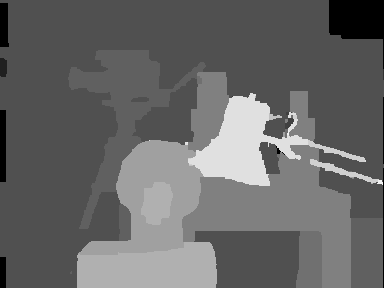
\includegraphics{pics/disparity.png}

\cvCPyFunc{POSIT}
Implements the POSIT algorithm.

\cvcodeC{
void cvPOSIT( \par CvPOSITObject* posit\_object,\par CvPoint2D32f* image\_points,\par double focal\_length,\par CvTermCriteria criteria,\par CvMatr32f rotation\_matrix,\par CvVect32f translation\_vector );
}\cvcodePy{POSIT(posit\_object,image\_points,focal\_length,criteria)-> rotation\_matrix,translation\_vector}

\begin{description}
\cvarg{posit\_object}{Pointer to the object structure}
\cvarg{image\_points}{Pointer to the object points projections on the 2D image plane}
\cvarg{focal\_length}{Focal length of the camera used}
\cvarg{criteria}{Termination criteria of the iterative POSIT algorithm}
\cvarg{rotation\_matrix}{Matrix of rotations}
\cvarg{translation\_vector}{Translation vector}
\end{description}

The function implements the POSIT algorithm. Image coordinates are given in a camera-related coordinate system. The focal length may be retrieved using the camera calibration functions. At every iteration of the algorithm a new perspective projection of the estimated pose is computed.

Difference norm between two projections is the maximal distance between corresponding points. The parameter \texttt{criteria.epsilon} serves to stop the algorithm if the difference is small.

\ifC
\cvCPyFunc{ProjectPoints2}
Projects 3D points on to an image plane.

\cvcodeC{
void cvProjectPoints2( \par const CvMat* object\_points,\par const CvMat* rotation\_vector,\par const CvMat* translation\_vector,\par const CvMat* intrinsic\_matrix,\par const CvMat* distortion\_coeffs,\par CvMat* image\_points,\par CvMat* dpdrot=NULL,\par CvMat* dpdt=NULL,\par CvMat* dpdf=NULL,\par CvMat* dpdc=NULL,\par CvMat* dpddist=NULL );
}\cvcodePy{ProjectPoints2(object\_points,rotation\_vector,translation\_vector,intrinsic\_matrix,distortion\_coeffs, image\_points,dpdrot=NULL,dpdt=NULL,dpdf=NULL,dpdc=NULL,dpddist=NULL)-> None}

\begin{description}
\cvarg{object\_points}{The array of object points, 3xN or Nx3, where N is the number of points in the view}
\cvarg{rotation\_vector}{The rotation vector, 1x3 or 3x1}
\cvarg{translation\_vector}{The translation vector, 1x3 or 3x1}
\cvarg{intrinsic\_matrix}{The camera matrix $A = \vecthreethree{fx}{0}{cx}{0}{fy}{cy}{0}{0}{1} $}
\cvarg{distortion\_coeffs}{The vector of distortion coefficients, 4x1 or 1x4 $k_1, k_2, k_3, k_4$. If it is \texttt{NULL}, all of the distortion coefficients are considered 0's}
\cvarg{image\_points}{The output array of image points, 2xN or Nx2, where N is the total number of points in the view}
\cvarg{dpdrot}{Optional Nx3 matrix of derivatives of image points with respect to components of the rotation vector}
\cvarg{dpdt}{Optional Nx3 matrix of derivatives of image points with respect to components of the translation vector}
\cvarg{dpdf}{Optional Nx2 matrix of derivatives of image points with respect to $fx$ and $fy$}
\cvarg{dpdc}{Optional Nx2 matrix of derivatives of image points with respect to $cx$ and $cy$}
\cvarg{dpddist}{Optional Nx4 matrix of derivatives of image points with respect to distortion coefficients}
\end{description}

The function computes projections of 3D
points to the image plane given intrinsic and extrinsic camera
parameters. Optionally, the function computes jacobians - matrices
of partial derivatives of image points as functions of all the
input parameters with respect to the particular parameters, intrinsic and/or
extrinsic. The jacobians are used during the global optimization
in \cvCPyCross{CalibrateCamera2} and
\cvCPyCross{FindExtrinsicCameraParams2}. The
function itself is also used to compute back-projection error for with
current intrinsic and extrinsic parameters.

Note, that with intrinsic and/or extrinsic parameters set to special
values, the function can be used to compute just an extrinsic transformation
or just an intrinsic transformation (i.e. distortion of a sparse set
of points).

\cvCPyFunc{RQDecomp3x3}
Computes the `RQ' decomposition of 3x3 matrices.

\cvcodeC{
void cvRQDecomp3x3( \par const CvMat *matrixM,\par CvMat *matrixR,\par CvMat *matrixQ,\par CvMat *matrixQx=NULL,\par CvMat *matrixQy=NULL,\par CvMat *matrixQz=NULL,\par CvPoint3D64f *eulerAngles=NULL);
}\cvcodePy{RQDecomp3x3(matrixM, matrixR, matrixQ, matrixQx = None, matrixQy = None, matrixQz = None) -> eulerAngles}

\begin{description}
\cvarg{matrixM}{The 3x3 input matrix M}
\cvarg{matrixR}{The output 3x3 upper-triangular matrix R}
\cvarg{matrixQ}{The output 3x3 orthogonal matrix Q}
\cvarg{matrixQx}{Optional 3x3 rotation matrix around x-axis}
\cvarg{matrixQy}{Optional 3x3 rotation matrix around y-axis}
\cvarg{matrixQz}{Optional 3x3 rotation matrix around z-axis}
\cvarg{eulerAngles}{Optional 3 points containing the three Euler angles of rotation}
\end{description}

The function computes a RQ decomposition using the given rotations. This function is used in \cvCPyCross{DecomposeProjectionMatrix} to decompose the left 3x3 submatrix of a projection matrix into a calibration and a rotation matrix.

It optionally returns three rotation matrices, one for each axis, and the three Euler angles that could be used in OpenGL.


\cvCPyFunc{ReleasePOSITObject}
Deallocates a 3D object structure.

\cvcodeC{
void cvReleasePOSITObject( \par CvPOSITObject** posit\_object );
}

\begin{description}
\cvarg{posit\_object}{Double pointer to \texttt{CvPOSIT} structure}
\end{description}

The function releases memory previously allocated by the function \cvCPyCross{CreatePOSITObject}.

\fi

\cvCPyFunc{ReleaseStereoBMState}
Releases block matching stereo correspondence structure.

\cvcodeC{

void cvReleaseStereoBMState( CvStereoBMState** state );

}\cvcodePy{ReleaseStereoBMState(state)-> None}

\begin{description}
\cvarg{state}{Double pointer to the released structure.}
\end{description}

The function releases the stereo correspondence structure and all the associated internal buffers. 

\cvCPyFunc{ReleaseStereoGCState}
Releases the state structure of the graph cut-based stereo correspondence algorithm.

\cvcodeC{

void cvReleaseStereoGCState( CvStereoGCState** state );

}\cvcodePy{ReleaseStereoGCState(state)-> None}

\begin{description}
\cvarg{state}{Double pointer to the released structure.}
\end{description}

The function releases the stereo correspondence structure and all the associated internal buffers. 


\cvCPyFunc{Rodrigues2}
Converts a rotation matrix to a rotation vector or vice versa.

\cvcodeC{
int  cvRodrigues2( \par const CvMat* src,\par CvMat* dst,\par CvMat* jacobian=0 );
}\cvcodePy{Rodrigues2(src,dst,jacobian=0)-> None}

\begin{description}
\cvarg{src}{The input rotation vector (3x1 or 1x3) or rotation matrix (3x3)}
\cvarg{dst}{The output rotation matrix (3x3) or rotation vector (3x1 or 1x3), respectively}
\cvarg{jacobian}{Optional output Jacobian matrix, 3x9 or 9x3 - partial derivatives of the output array components with respect to the input array components}
\end{description}

The function converts a rotation vector to a rotation matrix or vice versa. A rotation vector is a compact representation of rotation matrix. Direction of the rotation vector is the rotation axis and the length of the vector is the rotation angle around the axis. The rotation matrix $R$, corresponding to the rotation vector $r$, is computed as following:

\[
\begin{array}{l}
\theta \leftarrow norm(r)\\
r \leftarrow r/\theta\\
R = \cos{\theta} I + (1-\cos{\theta}) r r^T + \sin{\theta}
\vecthreethree
{0}{-r_z}{r_y}
{r_z}{0}{-r_x}
{-r_y}{r_x}{0}
\end{array}
\]

Inverse transformation can also be done easily as

\[
\sin(\theta)
\vecthreethree
{0}{-r_z}{r_y}
{r_z}{0}{-r_x}
{-r_y}{r_x}{0}
=
\frac{R - R^T}{2}
\]

A rotation vector is a convenient representation of a rotation matrix
as a matrix with only 3 degrees of freedom. The representation is
used in the global optimization procedures inside
\cvCPyCross{FindExtrinsicCameraParams2}
and \cvCPyCross{CalibrateCamera2}.


\cvCPyFunc{StereoCalibrate}
Calibrates stereo camera.

\cvcodeC{

void cvStereoCalibrate( \par const CvMat* object\_points, \par const CvMat* image\_points1,
                        \par const CvMat* image\_points2, \par const CvMat* point\_counts,
                        \par CvMat* camera\_matrix1, \par CvMat* dist\_coeffs1,
                        \par CvMat* camera\_matrix2, \par CvMat* dist\_coeffs2,
                       \par CvSize image\_size, \par CvMat* R, \par CvMat* T,
                        \par CvMat* E=0, \par CvMat* F=0,
                        \par CvTermCriteria term\_crit=cvTermCriteria(
                               \par CV\_TERMCRIT\_ITER+CV\_TERMCRIT\_EPS,30,1e-6),
                        \par int flags=CV\_CALIB\_FIX\_INTRINSIC );

}\cvcodePy{StereoCalibrate(\par object\_points,\par image\_points1,\par image\_points2,\par point\_counts,\par camera\_matrix1,\par dist\_coeffs1,\par camera\_matrix2,\par dist\_coeffs2,\par image\_size,\par R,\par T,\par E=NULL,\par F=NULL,\par term\_crit=cvTermCriteria(CV\_TERMCRIT\_ITER+CV\_TERMCRIT\_EPS,30,1e-6),\par flags=CV\_CALIB\_FIX\_INTRINSIC)-> None}

\begin{description}
\cvarg{object\_points}{The joint matrix of object points, 3xN or Nx3, where N is the total number of points in all views.}
\cvarg{image\_points1}{The joint matrix of corresponding image points in the views from the 1st camera, 2xN or Nx2, where N is the total number of points in all views.}
\cvarg{image\_points2}{The joint matrix of corresponding image points in the views from the 2nd camera, 2xN or Nx2, where N is the total number of points in all views.}
\cvarg{point\_counts}{Vector containing numbers of points in each view, 1xM or Mx1, where M is the number of views.}
\cvarg{camera\_matrix1, camera\_matrix2}{The input/output camera matrices [${fx}_k 0 {cx}_k; 0 {fy}_k {cy}_k; 0 0 1$]. If \texttt{CV\_CALIB\_USE\_INTRINSIC\_GUESS} or \texttt{CV\_CALIB\_FIX\_ASPECT\_RATIO} are specified, some or all of the elements of the matrices must be initialized.}
\cvarg{dist\_coeffs1, dist\_coeffs2}{The input/output vectors of distortion coefficients for each camera, \href{\#Pinhole Camera Model, Distortion}{4x1, 1x4, 5x1 or 1x5.}}
\cvarg{image\_size}{Size of the image, used only to initialize intrinsic camera matrix.} 
\cvarg{R}{The rotation matrix between the 1st and the 2nd cameras' coordinate systems.}
\cvarg{T}{The translation vector between the cameras' coordinate systems.}
\cvarg{E}{The optional output essential matrix.}
\cvarg{F}{The optional output fundamental matrix.}
\cvarg{term\_crit}{Termination criteria for the iterative optimiziation algorithm.}
\cvarg{flags}{Different flags, may be 0 or combination of the following values:
\begin{description}
\cvarg{CV\_CALIB\_FIX\_INTRINSIC}{If it is set, \texttt{camera\_matrix1,2}, as well as \texttt{dist\_coeffs1,2} are fixed, so that only extrinsic parameters are optimized.}
\cvarg{CV\_CALIB\_USE\_INTRINSIC\_GUESS}{The flag allows the function to optimize some or all of the intrinsic parameters, depending on the other flags, but the initial values are provided by the user.}
\cvarg{CV\_CALIB\_FIX\_PRINCIPAL\_POINT}{The principal points are fixed during the optimization.}
\cvarg{CV\_CALIB\_FIX\_FOCAL\_LENGTH}{${fx}_k$ and ${fy}_k$ are fixed.}
\cvarg{CV\_CALIB\_FIX\_ASPECT\_RATIO}{${fy}_k$ is optimized, but the ratio ${fx}_k/{fy}_k$ is fixed.}
\cvarg{CV\_CALIB\_SAME\_FOCAL\_LENGTH}{Enforces ${fx}_0={fx}_1$ and ${fy}_0={fy}_1$. \texttt{CV\_CALIB\_ZERO\_TANGENT\_DIST} - Tangential distortion coefficients for each camera are set to zeros and fixed there.}
\cvarg{CV\_CALIB\_FIX\_K1}{The 0-th distortion coefficients (k1) are fixed.}
\cvarg{CV\_CALIB\_FIX\_K2}{The 1-st distortion coefficients (k2) are fixed.}
\cvarg{CV\_CALIB\_FIX\_K3}{The 4-th distortion coefficients (k3) are fixed.}
\end{description}}
\end{description}

The function estimates transformation between the 2 cameras making a stereo pair. If we have a stereo camera, where the relative position and orientatation of the 2 cameras is fixed, and if we computed poses of an object relative to the fist camera and to the second camera, (R1, T1) and (R2, T2), respectively (that can be done with \cvCPyCross{cvFindExtrinsicCameraParams2}), obviously, those poses will relate to each other, i.e. given ($R_1$, $T_1$) it should be possible to compute ($R_2$, $T_2$) - we only need to know the position and orientation of the 2nd camera relative to the 1st camera. That's what the described function does. It computes ($R$, $T$) such that:

\[
R_2=R*R_1
T_2=R*T_1 + T,
\]

Optionally, it computes the essential matrix E:

\[
E=
\vecthreethree
{0}{-T_2}{T_1}
{T_2}{0}{-T_0}
{-T_1}{T_0}{0}
*R
\]

where $T_i$ are components of the translation vector $T$: $T=[T_0, T_1, T_2]^T$. And also the function can compute the fundamental matrix F:

$F = inv(camera\_matrix2)^T*E*inv(camera\_matrix1)$

Besides the stereo-related information, the function can also perform full calibration of each of the 2 cameras. However, because of the high dimensionality of the parameter space and noise in the input data the function can diverge from the correct solution. Thus, if intrinsic parameters can be estimated with high accuracy for each of the cameras individually (e.g. using \cvCPyCross{cvCalibrateCamera2}), it is recommended to do so and then pass \texttt{CV\_CALIB\_FIX\_INTRINSIC} flag to the function along with the computed intrinsic parameters. Otherwise, if all the parameters are estimated at once, it makes sense to restrict some parameters, e.g. pass \texttt{CV\_CALIB\_SAME\_FOCAL\_LENGTH} and \texttt{CV\_CALIB\_ZERO\_TANGENT\_DIST} flags, which are usually reasonable assumptions. 

\cvCPyFunc{StereoRectify}
Computes rectification transform for stereo camera.

\cvcodeC{

void cvStereoRectify( \par const CvMat* camera\_matrix1, \par const CvMat* camera\_matrix2,
                      \par const CvMat* dist\_coeffs1, \par const CvMat* dist\_coeffs2,
                      \par CvSize image\_size, \par const CvMat* R, \par const CvMat* T,
                      \par CvMat* R1, \par CvMat* R2, \par CvMat* P1, \par CvMat* P2,
                      \par CvMat* Q=0, \par int flags=CV\_CALIB\_ZERO\_DISPARITY );

}\cvcodePy{StereoRectify(\par camera\_matrix1,\par camera\_matrix2,\par dist\_coeffs1,\par dist\_coeffs2,\par image\_size,\par R,\par T,\par R1,\par R2,\par P1,\par P2,\par Q=NULL,\par flags=CV\_CALIB\_ZERO\_DISPARITY)-> None}

\begin{description}
\cvarg{camera\_matrix1, camera\_matrix2}{The camera matrices [${fx}_k$ 0 ${cx}_k$; 0 ${fy}_k$ ${cy}_k$; 0 0 1].}
\cvarg{dist\_coeffs1, dist\_coeffs2}{The vectors of distortion coefficients for each camera, \href{\#Pinhole Camera Model, Distortion}{4x1, 1x4, 5x1 or 1x5.}}
\cvarg{image\_size}{Size of the image used for stereo calibration.}
\cvarg{R}{The rotation matrix between the 1st and the 2nd cameras' coordinate systems.}
\cvarg{T}{The translation vector between the cameras' coordinate systems.}
\cvarg{R1, R2}{3x3 Rectification transforms (rotation matrices) for the first and the second cameras, respectively.}
\cvarg{P1, P2}{3x4 Projection matrices in the new (rectified) coordinate systems.}
\cvarg{Q}{The optional output disparity-to-depth mapping matrix, 4x4, see \cvCPyCross{cvReprojectImageTo3D}.}
\cvarg{flags}{The operation flags; may be 0 or \texttt{CV\_CALIB\_ZERO\_DISPARITY}. If the flag is set, the function makes the principal points of each camera have the same pixel coordinates in the rectified views. And if the flag is not set, the function can shift one of the image in horizontal or vertical direction (depending on the orientation of epipolar lines) in order to maximise the useful image area. }
\end{description}

The function computes the rotation matrices for each camera that (virtually) make both camera image planes the same plane. Consequently, that makes all the epipolar lines parallel and thus simplifies the dense stereo correspondence problem. On input the function takes the matrices computed by \cvCPyCross{cvStereoCalibrate} and on output it gives 2 rotation matrices and also 2 projection matrices in the new coordinates. The function is normally called after \cvCPyCross{cvStereoCalibrate} that computes both camera matrices, the distortion coefficients, R and T. The 2 cases are distinguished by the function: 

\begin{enumerate}
\item{Horizontal stereo, when 1st and 2nd camera views are shifted relative to each other mainly along the x axis (with possible small vertical shift). Then in the rectified images the corresponding epipolar lines in left and right cameras will be horizontal and have the same y-coordinate. P1 and P2 will look as: 

\[
P1=
\begin{array}{cccc}
f & 0 & cx1 & 0\\
0 & f & cy & 0\\
0 & 0 & 1 & 0
\end{array}
\]
\[
P2=
\begin{array}{cccc}
f & 0 & cx2 & Tx*f\\
0 & f & cy & 0\\
0 & 0 & 1 & 0
\end{array}
,
\]

where $T_x$ is horizontal shift between the cameras and cx1=cx2 if \texttt{CV\_CALIB\_ZERO\_DISPARITY} is set.}
\item{Vertical stereo, when 1st and 2nd camera views are shifted relative to each other mainly in vertical direction (and probably a bit in the horizontal direction too). Then the epipolar lines in the rectified images will be vertical and have the same x coordinate. P2 and P2 will look as:

\[
P1=
\begin{array}{cccc}
f & 0 & cx & 0\\
0 & f & cy1 & 0\\
0 & 0 & 1 & 0
\end{array}
\]
\[
P2=
\begin{array}{cccc}
f & 0 & cx & 0\\
0 & f & cy2 & Ty*f\\
0 & 0 & 1 & 0
\end{array}
,
\]

where $T_y$ is vertical shift between the cameras and cy1=cy2 if \texttt{CV\_CALIB\_ZERO\_DISPARITY} is set.}
\end{enumerate} 

As you can see, the first 3 columns of P1 and P2 will effectively be the new "rectified" camera matrices. 

\cvCPyFunc{StereoRectifyUncalibrated}
Computes rectification transform for uncalibrated stereo camera.

\cvcodeC{

void cvStereoRectifyUncalibrated( \par const CvMat* points1, \par const CvMat* points2,
                                  \par const CvMat* F, \par CvSize image\_size,
                                  \par CvMat* H1, \par CvMat* H2,
                                  \par double threshold=5 );

}\cvcodePy{StereoRectifyUncalibrated(points1,points2,F,image\_size,H1,H2,threshold=5)-> None}

\begin{description}
\cvarg{points1, points2}{The 2 arrays of corresponding 2D points.}
\cvarg{F}{Fundamental matrix. It can be computed using the same set of point pairs points1 and points2  using \cvCPyCross{cvFindFundamentalMat}.}
\cvarg{image\_size}{Size of the image.}
\cvarg{H1, H2}{The rectification homography matrices for the first and for the second images.}
\cvarg{threshold}{Optional threshold used to filter out the outliers. If the parameter is greater than zero, then all the point pairs that do not comply the epipolar geometry well enough (that is, the points for which $fabs(points2[i]^T*F*points1[i])>threshold$) are rejected prior to computing the homographies. }
\end{description}

The function computes the rectification transformations without knowing intrinsic parameters of the cameras and their relative position in space, hence the suffix "Uncalibrated". Another related difference from \cvCPyCross{cvStereoRectify} is that the function outputs not the rectification transformations in the object (3D) space, but the planar perspective transformations, encoded by the homography matrices H1 and H2. The function implements the following algorithm \href{\#Hartly99}{[Hartley99]}. 

Note that while the algorithm does not need to know the intrinsic parameters of the cameras, it heavily depends on the epipolar geometry. Therefore, if the camera lenses have significant distortion, it would better be corrected before computing the fundamental matrix and calling this function. For example, distortion coefficients can be estimated for each head of stereo camera separately by using \cvCPyCross{cvCalibrateCamera2} and then the images can be corrected using \cvCPyCross{cvUndistort2}. 

\cvCPyFunc{UndistortPoints}
Computes the ideal point coordinates from the observed point coordinates.

\cvcodeC{

void cvUndistortPoints( \par const CvMat* src, \par CvMat* dst,
                        \par const CvMat* camera\_matrix,
                        \par const CvMat* dist\_coeffs,
                        \par const CvMat* R=NULL,
                        \par const CvMat* P=NULL);

}\cvcodePy{UndistortPoints(src,dst,camera\_matrix,dist\_coeffs,R=NULL,P=NULL)-> None}

\begin{description}
\cvarg{src}{The observed point coordinates}
\cvarg{dst}{The ideal point coordinates, after undistortion and reverse perspective transformation}
\cvarg{camera\_matrix}{The camera matrix $A=[fx 0 cx; 0 fy cy; 0 0 1]$}
\cvarg{dist\_coeffs}{he vector of distortion coefficients, \cvCPyCross{4x1, 1x4, 5x1 or 1x5}}
\cvarg{R}{The rectification transformation in object space (3x3 matrix). \texttt{R1} or \texttt{R2}, computed by \cvCPyCross{StereoRectify} can be passed here. If the parameter is NULL, the identity matrix is used}
\cvarg{P}{The new camera matrix (3x3) or the new projection matrix (3x4). \texttt{P1} or \texttt{P2}, computed by \cvCPyCross{StereoRectify} can be passed here. If the parameter is NULL, the identity matrix is used}
\end{description}

The function is similar to \cvCPyCross{InitUndistortRectifyMap} and is opposite to it at the same time. The functions are similar in that they both are used to correct lens distortion and to perform the optional perspective (rectification) transformation. They are opposite because the function \cvCPyCross{InitUndistortRectifyMap} does actually perform the reverse transformation in order to initialize the maps properly, while this function does the forward transformation. That is, in pseudo-code it can be expressed as:

\begin{lstlisting}
// (u,v) is the input point, (u', v') is the output point
// camera_matrix=[fx 0 cx; 0 fy cy; 0 0 1]
// P=[fx' 0 cx' tx; 0 fy' cy' ty; 0 0 1 tz]
x" = (u - cx)/fx
y" = (v - cy)/fy
(x',y') = undistort(x",y",dist_coeffs)
[X,Y,W]T = R*[x' y' 1]T
x = X/W, y = Y/W
u' = x*fx' + cx'
v' = y*fy' + cy',
\end{lstlisting}

where undistort() is approximate iterative algorithm that estimates the normalized original point coordinates out of the normalized distorted point coordinates ("normalized" means that the coordinates do not depend on the camera matrix).

The function can be used as for stereo cameras, as well as for individual cameras when R=NULL. 

\fi


\ifCpp

\cvCppFunc{calibrateCamera}
Finds the camera matrix and the camera poses from several views of the calibration pattern.

\begin{lstlisting}
void calibrateCamera( const vector<vector<Point3f> >& objectPoints,
                      const vector<vector<Point2f> >& imagePoints,
                      Size imageSize,
                      Mat& cameraMatrix, Mat& distCoeffs,
                      vector<Mat>& rvecs, vector<Mat>& tvecs,
                      int flags=0 );
enum
{
  CALIB_USE_INTRINSIC_GUESS = CV_CALIB_USE_INTRINSIC_GUESS,
  CALIB_FIX_ASPECT_RATIO = CV_CALIB_FIX_ASPECT_RATIO,
  CALIB_FIX_PRINCIPAL_POINT = CV_CALIB_FIX_PRINCIPAL_POINT,
  CALIB_ZERO_TANGENT_DIST = CV_CALIB_ZERO_TANGENT_DIST,
  CALIB_FIX_FOCAL_LENGTH = CV_CALIB_FIX_FOCAL_LENGTH,
  CALIB_FIX_K1 = CV_CALIB_FIX_K1,
  CALIB_FIX_K2 = CV_CALIB_FIX_K2,
  CALIB_FIX_K3 = CV_CALIB_FIX_K3,
  // only for stereo
  CALIB_FIX_INTRINSIC = CV_CALIB_FIX_INTRINSIC,
  CALIB_SAME_FOCAL_LENGTH = CV_CALIB_SAME_FOCAL_LENGTH,
  // for stereo rectification
  CALIB_ZERO_DISPARITY = CV_CALIB_ZERO_DISPARITY
};
\end{lstlisting}

\begin{description}
\cvarg{objectPoints}{The vector of vectors of points on the calibration rig in its coordinate system, one vector per a view of the rig. If the the same calibration rig is shown in each view and it's fully visible, all the vectors can be the same (though, you may change the numbering from one view to another). The points are 3D, but since they are in the rig coordinate system, then if the rig is planar, it may have sense to put the model to the XY coordinate plane, so that Z-coordinate of each input object point is 0}
\cvarg{imagePoints}{The vector of vectors of the object point projections on the calibration rig views, one vector per a view. The projections must be in the same order as the corresponding object points.}
\cvarg{imageSize}{Size of the image, used only to initialize the intrinsic camera matrix}
\cvarg{cameraMatrix}{The input/output matrix of intrinsic camera parameters $A = \vecthreethree{fx}{0}{cx}{0}{fy}{cy}{0}{0}{1}$. If any of \texttt{CALIB\_USE\_INTRINSIC\_GUESS}, \texttt{CALIB\_FIX\_ASPECT\_RATIO}, \texttt{CALIB\_FIX\_FOCAL\_LENGTH} are specified, some or all of \texttt{fx, fy, cx, cy} must be initialized}
\cvarg{distCoeffs}{The input/output lens distortion coefficients, 4x1, 5x1, 1x4 or 1x5 floating-point vector $k_1, k_2, p_1, p_2[, k_3]$. If any of \texttt{CALIB\_FIX\_K1}, \texttt{CALIB\_FIX\_K2} or \texttt{CALIB\_FIX\_K3} is specified, then the corresponding elements of \texttt{distCoeffs} must be initialized.}
\cvarg{rvecs}{The output vector of rotation vectors (see \cvCppCross{Rodrigues}) estimated for each camera view}
\cvarg{tvecsrans}{The output vector of translation vectors estimated for each camera view}
\cvarg{flags}{Different flags, may be 0 or a combination of the following values:
\begin{description}
\cvarg{CALIB\_USE\_INTRINSIC\_GUESS}{\texttt{cameraMatrix} contains the valid initial values of \texttt{fx, fy, cx, cy} that are optimized further. Otherwise, \texttt{(cx, cy)} is initially set to the image center (computed from the input \texttt{imageSize}), and focal distances are computed in some least-squares fashion. Note, that if the focal distance initialization is currently supported only for planar calibration rigs. That is, if the calibration rig is 3D, then you must initialize \texttt{cameraMatrix} and pass \texttt{CALIB\_USE\_INTRINSIC\_GUESS} flag. Also, note that distortion coefficients are not regulated by this function; use \texttt{CALIB\_ZERO\_TANGENT\_DIST} and \texttt{CALIB\_FIX\_K?} to fix them}
\cvarg{CALIB\_FIX\_PRINCIPAL\_POINT}{The principal point is not changed during the global optimization, it stays at the center or, when \texttt{CALIB\_USE\_INTRINSIC\_GUESS} is set too, at the other specified location}
\cvarg{CALIB\_FIX\_ASPECT\_RATIO}{The optimization procedure considers only one of \texttt{fx} and \texttt{fy} as independent variables and keeps the aspect ratio \texttt{fx/fy} the same as it was set initially in the input \texttt{cameraMatrix}. In this case the actual initial values of \texttt{(fx, fy)} are either taken from the matrix (when \texttt{CALIB\_USE\_INTRINSIC\_GUESS} is set) or estimated.}
\cvarg{CALIB\_ZERO\_TANGENT\_DIST}{Tangential distortion coefficients are set to zeros and do not change during the optimization.}
\cvarg{CALIB\_FIX\_FOCAL\_LENGTH}{Both \texttt{fx} and \texttt{fy} are fixed (taken from \texttt{cameraMatrix} and do not change during the optimization.}
\cvarg{CALIB\_FIX\_K1, CALIB\_FIX\_K2, CALIB\_FIX\_K3}{The particular distortion coefficients is read from the input \texttt{distCoeffs} and stays the same during optimization}
\end{description}}
\end{description}

The function estimates the intrinsic camera
parameters and the extrinsic parameters for each of the views. The
coordinates of 3D object points and their correspondent 2D projections
in each view must be specified. You can use a calibration rig with a known geometry and easily and precisely detectable feature points, e.g. a checkerboard (see \cvCppCross{findChessboardCorners}).

The algorithm does the following:
\begin{enumerate}
    \item First, it computes the initial intrinsic parameters (only for planar calibration rigs) or reads them from the input parameters. The distortion coefficients are all set to zeros initially (unless some of \texttt{CALIB\_FIX\_K?} are specified).
    \item The the initial camera pose is estimated as if the intrinsic parameters have been already known. This is done using \cvCppCross{solvePnP}
    \item After that the global Levenberg-Marquardt optimization algorithm is run to minimize the reprojection error, i.e. the total sum of squared distances between the observed feature points \texttt{imagePoints} and the projected (using the current estimates for camera parameters and the poses) object points \texttt{objectPoints}; see \cvCppCross{projectPoints}.
\end{enumerate}

Note: if you're using a non-square (=non-NxN) grid and
\cvCppCross{findChessboardCorners} for calibration, and \texttt{calibrateCamera} returns
bad values (i.e. zero distortion coefficients, an image center very far from
$(w/2-0.5,h/2-0.5)$, and / or large differences between $f_x$ and $f_y$ (ratios of
10:1 or more)), then you've probaby used \texttt{patternSize=cvSize(rows,cols)},
but should use \texttt{patternSize=cvSize(cols,rows)} in \cvCppCross{findChessboardCorners}.

See also: \cvCppCross{findChessboardCorners}, \cvCppCross{solvePnP}, \cvCppCross{initCameraMatrix2D}, \cvCppCross{stereoCalibrate}, \cvCppCross{undistort}


\cvCppFunc{calibrationMatrixValues}
Computes some useful camera characteristics from the camera matrix

\begin{lstlisting}
void calibrationMatrixValues( const Mat& cameraMatrix,
                              Size imageSize,
                              double apertureWidth,
                              double apertureHeight,
                              double& fovx,
                              double& fovy,
                              double& focalLength,
                              Point2d& principalPoint,
                              double& aspectRatio );
\end{lstlisting}
\begin{description}
\cvarg{cameraMatrix}{The input camera matrix that can be estimated by \cvCppCross{calibrateCamera} or \cvCppCross{stereoCalibrate}}
\cvarg{imageSize}{The input image size in pixels}
\cvarg{apertureWidth}{Physical width of the sensor}
\cvarg{apertureHeight}{Physical height of the sensor}
\cvarg{fovx}{The output field of view in degrees along the horizontal sensor axis}
\cvarg{fovy}{The output field of view in degrees along the vertical sensor axis}
\cvarg{focalLength}{The focal length of the lens in mm}
\cvarg{prinicialPoint}{The principal point in pixels}
\cvarg{aspectRatio}{$f_y/f_x$}
\end{description}

The function computes various useful camera characteristics from the previously estimated camera matrix.

\cvCppFunc{composeRT}
Combines two rotation-and-shift transformations

\begin{lstlisting}
void composeRT( const Mat& rvec1, const Mat& tvec1,
                const Mat& rvec2, const Mat& tvec2,
                Mat& rvec3, Mat& tvec3 );
                
void composeRT( const Mat& rvec1, const Mat& tvec1,
                const Mat& rvec2, const Mat& tvec2,
                Mat& rvec3, Mat& tvec3,
                Mat& dr3dr1, Mat& dr3dt1,
                Mat& dr3dr2, Mat& dr3dt2,
                Mat& dt3dr1, Mat& dt3dt1,
                Mat& dt3dr2, Mat& dt3dt2 );
\end{lstlisting}
\begin{description}
\cvarg{rvec1}{The first rotation vector}
\cvarg{tvec1}{The first translation vector}
\cvarg{rvec2}{The second rotation vector}
\cvarg{tvec2}{The second translation vector}
\cvarg{rvec3}{The output rotation vector of the superposition}
\cvarg{tvec3}{The output translation vector of the superposition}
\cvarg{d??d??}{The optional output derivatives of \texttt{rvec3} or \texttt{tvec3} w.r.t. \texttt{rvec?} or \texttt{tvec?}}
\end{description}

The functions compute:

\[ \begin{array}{l}
\texttt{rvec3} = \mathrm{rodrigues}^{-1}\left(\mathrm{rodrigues}(\texttt{rvec2}) \cdot
\mathrm{rodrigues}(\texttt{rvec1})\right) \\
\texttt{tvec3} = \mathrm{rodrigues}(\texttt{rvec2}) \cdot \texttt{tvec1} + \texttt{tvec2}
\end{array}, \]

where $\mathrm{rodrigues}$ denotes a rotation vector to rotation matrix transformation, and $\mathrm{rodrigues}^{-1}$ denotes the inverse transformation, see \cvCppCross{Rodrigues}.

Also, the functions can compute the derivatives of the output vectors w.r.t the input vectors (see \cvCppCross{matMulDeriv}).
The functions are used inside \cvCppCross{stereoCalibrate} but can also be used in your own code where Levenberg-Marquardt or another gradient-based solver is used to optimize a function that contains matrix multiplication.


\cvCppFunc{computeCorrespondEpilines}
For points in one image of a stereo pair, computes the corresponding epilines in the other image.

\begin{lstlisting}
void computeCorrespondEpilines( const Mat& points,
                                int whichImage, const Mat& F,
                                vector<Vec3f>& lines );
\end{lstlisting}
\begin{description}
\cvarg{points}{The input points. $N \times 1$ or $1 \times N$ matrix of type \texttt{CV\_32FC2} or \texttt{vector<Point2f>}}
\cvarg{whichImage}{Index of the image (1 or 2) that contains the \texttt{points}}
\cvarg{F}{The fundamental matrix that can be estimated using \cvCppCross{findFundamentalMat} or \texttt{stereoRectify}}
\cvarg{lines}{The output vector of the corresponding to the points epipolar lines in the other image. Each line $ax + by + c=0$ is encoded as 3-element vector $(a, b, c)$}
\end{description}

For every point in one of the two images of a stereo-pair the function
\texttt{computeCorrespondEpilines} finds the equation of the
corresponding epipolar line in the other image.

From the fundamental matrix definition (see \cvCppCross{findFundamentalMatrix}),
line $l^{(2)}_i$ in the second image for the point $p^{(1)}_i$ in the first image (i.e. when \texttt{whichImage=1}) is computed as:

\[ l^{(2)}_i = F p^{(1)}_i \]

and, vice versa, when \texttt{whichImage=2}, $l^{(1)}_i$ is computed from $p^{(2)}_i$ as:

\[ l^{(1)}_i = F^T p^{(2)}_i \]

Line coefficients are defined up to a scale. They are normalized, such that $a_i^2+b_i^2=1$.

\cvCppFunc{convertPointHomogeneous}
Converts 2D points to/from homogeneous coordinates.

\begin{lstlisting}
void convertPointsHomogeneous( const Mat& src, vector<Point3f>& dst );
void convertPointsHomogeneous( const Mat& src, vector<Point2f>& dst );
\end{lstlisting}
\cvarg{src}{The input array or vector of 2D or 3D points}
\cvarg{dst}{The output vector of 3D or 2D points, respectively}
\end{description}

The first of the functions converts 2D points to the homogeneous coordinates by adding extra \texttt{1} component to each point. When the input vector already contains 3D points, it is simply copied to \texttt{dst}. The second function converts 3D points to 2D points by dividing 1st and 2nd components by the 3rd one. If the input vector already contains 2D points, it is simply copied to \texttt{dst}.

\cvCppFunc{decomposeProjectionMatrix}
Decomposes the projection matrix into a rotation matrix and a camera matrix.

\begin{lstlisting}
void decomposeProjectionMatrix( const Mat& projMatrix, Mat& cameraMatrix,
                                Mat& rotMatrix, Mat& transVect );
void decomposeProjectionMatrix( const Mat& projMatrix, Mat& cameraMatrix,
                                Mat& rotMatrix, Mat& transVect,
                                Mat& rotMatrixX, Mat& rotMatrixY,
                                Mat& rotMatrixZ, Vec3d& eulerAngles );
\end{lstlisting}
\begin{description}
\cvarg{projMatrix}{The input $3 \times 4$ projection matrix}
\cvarg{cameraMatrix}{The output $3 \times 3$ camera matrix}
\cvarg{rotMatrix}{The output $3 \times 3$ rotation matrix}
\cvarg{transVect}{The output $3 \times 1$ translation vector}
\cvarg{rotMatrixX}{The optional output rotation matrix around x-axis}
\cvarg{rotMatrixY}{The optional output rotation matrix around y-axis}
\cvarg{rotMatrixZ}{The optional output rotation matrix around z-axis}
\cvarg{eulerAngles}{The optional output 3-vector of the Euler rotation angles}
\end{description}

The function computes a decomposition of a projection matrix into a calibration and a rotation matrix and the position of the camera.

It optionally returns three rotation matrices, one for each axis, and the three Euler angles that could be used in OpenGL.

The function is based on \cvCppCross{RQDecomp3x3}.

\cvCppFunc{drawChessboardCorners}
Draws the detected chessboard corners.

\begin{lstlisting}
void drawChessboardCorners( Mat& image, Size patternSize,
                            const Mat& corners,
                            bool patternWasFound );
\end{lstlisting}
\begin{description}
\cvarg{image}{The destination image; it must be an 8-bit color image}
\cvarg{patternSize}{The number of inner corners per chessboard row and column, i.e. \texttt{Size(<corners per row>, <corners per column>)}}
\cvarg{corners}{The array of detected corners; \texttt{vector<Point2f>} can be passed here as well}
\cvarg{patternWasFound}{Indicates whether the complete board was found. Just pass the return value of \cvCppCross{findChessboardCorners} here}
\end{description}

The function draws the detected chessboard corners. If no complete board was found, the detected corners will be marked with small red circles. Otherwise, a colored board (each board row with a different color) will be drawn.

\cvCppFunc{findFundamentalMat}
Calculates the fundamental matrix from the corresponding points in two images.

\begin{lstlisting}
Mat findFundamentalMat( const Mat& points1, const Mat& points2,
                        vector<uchar>& mask, int method=FM_RANSAC,
                        double param1=3., double param2=0.99 );

Mat findFundamentalMat( const Mat& points1, const Mat& points2,
                        int method=FM_RANSAC,
                        double param1=3., double param2=0.99 );
                        
enum
{ 
    FM_7POINT = CV_FM_7POINT,
    FM_8POINT = CV_FM_8POINT,
    FM_LMEDS = CV_FM_LMEDS,
    FM_RANSAC = CV_FM_RANSAC
};
\end{lstlisting}
\begin{description}
\cvarg{points1}{Array of $N$ points in the first image, a matrix of \texttt{CV\_32FC2} type or \texttt{vector<Point2f>}. The points in homogeneous coordinates can also be passed.}
\cvarg{points2}{Array of the corresponding points in the second image of the same size and the same type as \texttt{points1}}
\cvarg{method}{Method for computing the fundamental matrix
\begin{description}
  \cvarg{FM\_7POINT}{for a 7-point algorithm. $N = 7$}
  \cvarg{FM\_8POINT}{for an 8-point algorithm. $N \ge 8$}
  \cvarg{FM\_RANSAC}{for the RANSAC algorithm. $N \ge 8$}
  \cvarg{FM\_LMEDS}{for the LMedS algorithm. $N \ge 8$}
\end{description}}
\cvarg{param1}{The parameter is used for RANSAC only. It is the maximum distance in pixels from point to epipolar line in pixels, beyond which the point is considered an outlier and is not used for computing the final fundamental matrix. It can be set to something like 1-3, depending on the accuracy of the point localization, image resolution and the image noise}
\cvarg{param2}{The parameter is used for RANSAC or LMedS methods only. It denotes the desirable level of confidence (between 0 and 1) that the estimated matrix is correct}
\cvarg{mask}{The optional output array of $N$ elements, every element of which is set to 0 for outliers and to 1 for the other points. The array is computed only in RANSAC and LMedS methods. Other methods set every element to 1}
\end{description}

The epipolar geometry is described by the following equation:

\[ [p_2; 1]^T F [p_1; 1] = 0 \]

where $F$ is fundamental matrix, $p_1$ and $p_2$ are corresponding points in the first and the second images, respectively.

The function calculates the fundamental
matrix using one of four methods listed above and returns the found fundamental matrix. In the case of \texttt{FM\_7POINT} the function may return a $9 \times 3$ matrix. It means that the 3 fundamental matrices are possible and they are all found and stored sequentially.

The calculated fundamental matrix may be passed further to
\texttt{computeCorrespondEpilines} that finds the epipolar lines
corresponding to the specified points. It can also be passed to \cvCppCross{stereoRectifyUncalibrated} to compute the rectification transformation.

\begin{lstlisting}
// Example. Estimation of fundamental matrix using RANSAC algorithm
int point_count = 100;
vector<Point2f> points1(point_count);
vector<Point2f> points2(point_count);

// initialize the points here ... */
for( int i = 0; i < point_count; i++ )
{
    points1[i] = ...;
    points2[i] = ...;
}

Mat fundamental_matrix =
 findFundamentalMat(points1, points2, FM_RANSAC, 3, 0.99);
\end{lstlisting}


\cvCppFunc{findChessboardCorners}
Finds the positions of the internal corners of the chessboard.

\begin{lstlisting}
bool findChessboardCorners( const Mat& image, Size patternSize,
                            vector<Point2f>& corners,
                            int flags=CV_CALIB_CB_ADAPTIVE_THRESH+
                                 CV_CALIB_CB_NORMALIZE_IMAGE );
enum { CALIB_CB_ADAPTIVE_THRESH = CV_CALIB_CB_ADAPTIVE_THRESH,
    CALIB_CB_NORMALIZE_IMAGE = CV_CALIB_CB_NORMALIZE_IMAGE,
    CALIB_CB_FILTER_QUADS = CV_CALIB_CB_FILTER_QUADS };
\end{lstlisting}
\begin{description}
\cvarg{image}{The input chessboard (a.k.a. checkerboard) view; it must be an 8-bit grayscale or color image}
\cvarg{patternSize}{The number of inner corners per chessboard row and column, i.e.
\texttt{patternSize = cvSize(<points per row>, <points per column>)}}
\cvarg{corners}{The output vector of the corners detected. If the board is found (the function returned true), the corners should be properly ordered.}
\cvarg{flags}{Various operation flags, can be 0 or a combination of the following values:
\begin{description}
 \cvarg{CALIB\_CB\_ADAPTIVE\_THRESH}{use adaptive thresholding, instead of a fixed-level threshold, to convert the image to black and white rather than a fixed threshold level}
 \cvarg{CALIB\_CB\_NORMALIZE\_IMAGE}{normalize the image brightness and contrast using \cvCppCross{equalizeHist} before applying fixed or adaptive thresholding}
 \cvarg{CALIB\_CB\_FILTER\_QUADS}{use some additional criteria (like contour area, perimeter, square-like shape) to filter out false quads that are extracted at the contour retrieval stage. Since the current corner grouping engine is smart enough, usually this parameter is omitted.}
\end{description}}
\end{description}

The function attempts to determine
whether the input image is a view of the chessboard pattern and, if yes,
locate the internal chessboard corners. The function returns true if all
of the chessboard corners have been found and they have been placed
in a certain order (row by row, left to right in every row),
otherwise, if the function fails to find all the corners or reorder
them, it returns 0. For example, a regular chessboard has 8 x 8
squares and 7 x 7 internal corners, that is, points, where the black
squares touch each other. The coordinates detected are approximate,
and to determine their position more accurately, the user may use
the function \cvCppCross{cornerSubPix} or other subpixel adjustment technique.

Sometimes the function fails to find the board because the image is too large or too small. If so, try to resize it and then scale the found corners coordinates back (or even scale the computed \texttt{cameraMatrix} back).


\cvCppFunc{getDefaultNewCameraMatrix}
Returns the default new camera matrix

\begin{lstlisting}
Mat getDefaultNewCameraMatrix( const Mat& cameraMatrix, Size imgSize=Size(),
                               bool centerPrincipalPoint=false );
\end{lstlisting}
\begin{description}
\cvarg{cameraMatrix}{The input camera matrix}
\cvarg{imageSize}{The camera view image size in pixels}
\cvarg{centerPrincipalPoint}{Indicates whether in the new camera matrix the principal point should be at the image center or not}
\end{description}

The function returns the camera matrix that is either an exact copy of the input \texttt{cameraMatrix} (when \texttt{centerPrinicipalPoint=false}), or the modified one (when \texttt{centerPrincipalPoint}=true).

In the latter case the new camera matrix will be:

\[\begin{bmatrix}
f_x && 0 && (\texttt{imgSize.width}-1)*0.5 \\
0 && f_y && (\texttt{imgSize.height}-1)*0.5 \\
0 && 0 && 1
\end{bmatrix},\]

where $f_x$ and $f_y$ are $(0,0)$ and $(1,1)$ elements of \texttt{cameraMatrix}, respectively.

By default, the undistortion functions in OpenCV (see \texttt{initUndistortRectifyMap}, \texttt{undistort}) do not move the principal point. However, when you work with stereo, it's important to move the principal points in both views to the same y-coordinate (which is required by most of stereo correspondence algorithms), and maybe to the same x-coordinate too. So you can form the new camera matrix for each view, where the principal points will be at the center. 

\cvCppFunc{initCameraMatrix2D}
Finds the initial camera matrix from the 3D-2D point correspondences

\begin{lstlisting}
Mat initCameraMatrix2D( const vector<vector<Point3f> >& objectPoints,
                        const vector<vector<Point2f> >& imagePoints,
                        Size imageSize, double aspectRatio=1. );
\end{lstlisting}
\begin{description}
\cvarg{objectPoints}{The vector of vectors of the object points. See \cvCppCross{calibrateCamera}}
\cvarg{imagePoints}{The vector of vectors of the corresponding image points. See \cvCppCross{calibrateCamera}}
\cvarg{imageSize}{The image size in pixels; used to initialize the principal point}
\cvarg{aspectRatio}{If it is zero or negative, both $f_x$ and $f_y$ are estimated independently. Otherwise $f_x = f_y * \texttt{aspectRatio}$}
\end{description}

The function estimates and returns the initial camera matrix for camera calibration process.
Currently, the function only supports planar calibration rigs, i.e. the rig for which the $3 \times 3$ covariance matrix of object points is singular.


\cvCppFunc{Rodrigues}
Converts a rotation matrix to a rotation vector or vice versa.

\begin{lstlisting}
void Rodrigues(const Mat& src, Mat& dst);
void Rodrigues(const Mat& src, Mat& dst, Mat& jacobian);
\end{lstlisting}

\begin{description}
\cvarg{src}{The input rotation vector (3x1 or 1x3) or a rotation matrix (3x3)}
\cvarg{dst}{The output rotation matrix (3x3) or a rotation vector (3x1 or 1x3), respectively}
\cvarg{jacobian}{The optional output Jacobian matrix, 3x9 or 9x3 - partial derivatives of the output array components with respect to the input array components}
\end{description}

The functions convert a rotation vector to a rotation matrix or vice versa. A rotation vector is a compact representation of rotation matrix. Direction of the rotation vector is the rotation axis and the length of the vector is the rotation angle around the axis. The rotation matrix $R$, corresponding to the rotation vector $r$, is computed as following:

\[
\begin{array}{l}
\theta \leftarrow norm(r)\\
r \leftarrow r/\theta\\
R = \cos{\theta} I + (1-\cos{\theta}) r r^T + \sin{\theta}
\vecthreethree
{0}{-r_z}{r_y}
{r_z}{0}{-r_x}
{-r_y}{r_x}{0}
\end{array}
\]

Inverse transformation can also be done easily, since

\[
\sin(\theta)
\vecthreethree
{0}{-r_z}{r_y}
{r_z}{0}{-r_x}
{-r_y}{r_x}{0}
=
\frac{R - R^T}{2}
\]

A rotation vector is a convenient and most-compact representation of a rotation matrix
(since any rotation matrix has just 3 degrees of freedom). The representation is
used in the global 3D geometry optimization procedures like \cvCppCross{calibrateCamera}, \cvCppCross{stereoCalibrate} or \cvCppCross{solvePnP}.


\cvCppFunc{RQDecomp3x3}
Computes the 'RQ' decomposition of 3x3 matrices.

\begin{lstlisting}
/* Computes RQ decomposition for 3x3 matrices */
void RQDecomp3x3( const Mat& M, Mat& R, Mat& Q );
Vec3d RQDecomp3x3( const Mat& M, Mat& R, Mat& Q,
                   Mat& Qx, Mat& Qy, Mat& Qz );
\end{lstlisting}
\begin{description}
\cvarg{M}{The input $3 \times 3$ floating-point matrix}
\cvarg{R}{The output $3 \times 3$ upper-triangular matrix}
\cvarg{Q}{The output $3 \times 3$ orthogonal matrix}
\cvarg{Qx, Qy, Qz}{The optional output matrices that decompose the rotation matrix Q into separate rotation matrices for each coordinate axis}
\end{description}

The function implements RQ decomposition of a $3 \times 3$ matrix. The function is by \cvCppCross{decomposeProjectionMatrix}.

\cvCppFunc{matMulDeriv}
Computes partial derivatives of the matrix product w.r.t each multiplied matrix

\begin{lstlisting}
void matMulDeriv( const Mat& A, const Mat& B, Mat& dABdA, Mat& dABdB );
\end{lstlisting}
\begin{description}
\cvarg{A}{The first multiplied matrix}
\cvarg{B}{The second multiplied matrix}
\cvarg{dABdA}{The first output derivative matrix \texttt{d(A*B)/dA} of size $\texttt{A.rows*B.cols} \times {A.rows*A.cols}$}
\cvarg{dABdA}{The second output derivative matrix \texttt{d(A*B)/dB} of size $\texttt{A.rows*B.cols} \times {B.rows*B.cols}$}
\end{description}

The function computes the partial derivatives of the elements of the matrix product $A*B$ w.r.t. the elements of each of the two input matrices. The function is used to compute Jacobian matrices in \cvCppCross{stereoCalibrate}, but can also be used in any other similar optimization function.

\cvCppFunc{projectPoints}
Projects 3D points on to an image plane.

\begin{lstlisting}
void projectPoints( const Mat& objectPoints,
                    const Mat& rvec, const Mat& tvec,
                    const Mat& cameraMatrix,
                    const Mat& distCoeffs,
                    vector<Point2f>& imagePoints );

void projectPoints( const Mat& objectPoints,
                    const Mat& rvec, const Mat& tvec,
                    const Mat& cameraMatrix,
                    const Mat& distCoeffs,
                    vector<Point2f>& imagePoints,
                    Mat& dpdrot, Mat& dpdt, Mat& dpdf,
                    Mat& dpdc, Mat& dpddist,
                    double aspectRatio=0 );
\end{lstlisting}
\begin{description}
\cvarg{objectPoints}{The input array of 3D object points, a matrix of type \texttt{CV\_32FC3} or \texttt{vector<Point3f>}}
\cvarg{imagePoints}{The output array of 2D image points}
\cvarg{rvec}{The rotation vector, 1x3 or 3x1}
\cvarg{tvec}{The translation vector, 1x3 or 3x1}
\cvarg{cameraMatrix}{The camera matrix $\vecthreethree{f_x}{0}{c_x}{0}{f_y}{c_y}{0}{0}{1}$}
\cvarg{distCoeffs}{The array of distortion coefficients, 4x1, 5x1, 1x4 or 1x5 $k_1, k_2, p_1, p_2[, k_3]$. If the matrix is empty, the function uses zero distortion coefficients}
\cvarg{dpdrot, dpdt, dpdf, dpdc, dpdist}{The optional matrices of the partial derivatives of the computed point projections w.r.t the rotation vector, the translation vector, $f_x$ and $f_y$, $c_x$ and $c_y$ and the distortion coefficients respectively. Each matrix has $2*N$ rows (where $N$ is the number of points) - even rows (0th, 2nd ...) are the derivatives of the x-coordinates w.r.t. the camera parameters and odd rows (1st, 3rd ...) are the derivatives of the y-coordinates.}
\cvarg{aspectRatio}{If zero or negative, $f_x$ and $f_y$ are treated as independent variables, otherwise they $f_x = f_y*\texttt{aspectRatio}$, so the derivatives are adjusted appropriately}
\end{description}

The function computes projections of 3D
points to the image plane given intrinsic and extrinsic camera
parameters. Optionally, the function computes jacobians - matrices
of partial derivatives of image points as functions of all the
input parameters with respect to the particular camera parameters, intrinsic and/or
extrinsic. The computed jacobians are used during the global optimization
in \cvCppCross{calibrateCamera}, \cvCppCross{stereoCalibrate} and \cvCppCross{solvePnP}.

Note, that by setting \texttt{rvec=tvec=(0,0,0)} or by setting \texttt{cameraMatrix=Mat::eye(3,3,CV\_64F)} or by setting \texttt{distCoeffs=Mat()} you can get various useful partial cases of the function, i.e. you can computed the distorted coordinates for a sparse set of points, or apply a perspective transformation (and also compute the derivatives) in the ideal zero-distortion setup etc.

\cvCppFunc{reprojectImageTo3D}
Reprojects disparity image to 3D space.

\begin{lstlisting}
void reprojectImageTo3D( const Mat& disparity,
                         Mat& _3dImage, const Mat& Q,
                         bool handleMissingValues=false );
\end{lstlisting}
\begin{description}
\cvarg{disparity}{The input single-channel 16-bit signed or 32-bit floating-point disparity image}
\cvarg{\_3dImage}{The output 3-channel floating-point image of the same size as \texttt{disparity}.
 Each element of \texttt{\_3dImage(x,y)} will contain the 3D coordinates of the point \texttt{(x,y)}, computed from the disparity map.}
\cvarg{Q}{The $4 \times 4$ perspective transformation matrix that can be obtained with \cvCppCross{stereoRectify}}
\cvarg{handleMissingValues}{If true, when the pixels with the minimal disparity (that corresponds to the ouliers; see \cvCppCross{StereoBM}) will be transformed to 3D points with some very large Z value (currently set to 10000)}
\end{description}
 
The function transforms 1-channel disparity map to 3-channel image representing a 3D surface. That is, for each pixel \texttt{(x,y)} and the corresponding disparity \texttt{d=disparity(x,y)} it computes: 

\[\begin{array}{l}
[X\; Y\; Z\; W]^T = \texttt{Q}*[x\; y\; \texttt{disparity}(x,y)\; 1]^T \\
\texttt{\_3dImage}(x,y) = (X/W,\; Y/W,\; Z/W)
\end{array}\]

The matrix \texttt{Q} can be arbitrary $4 \times 4$ matrix, e.g. the one computed by \cvCppCross{stereoRectify}. To reproject a sparse set of points {(x,y,d),...} to 3D space, use \cvCppCross{perspectiveTransform}.  


\cvCppFunc{solvePnP}
Finds the camera pose from the 3D-2D point correspondences

\begin{lstlisting}
void solvePnP( const Mat& objectPoints,
               const Mat& imagePoints,
               const Mat& cameraMatrix,
               const Mat& distCoeffs,
               Mat& rvec, Mat& tvec,
               bool useExtrinsicGuess=false );
\end{lstlisting}
\begin{description}
\cvarg{objectPoints}{The array of object points, a matrix of type \texttt{CV\_32FC3} or \texttt{vector<Point3f>}}
\cvarg{imagePoints}{The array of the corresponding image points, a matrix of type{CV\_32FC2} or \texttt{vector<Point2f>}}
\cvarg{cameraMatrix}{The input camera matrix $\vecthreethree{f_x}{0}{c_x}{0}{f_y}{c_y}{0}{0}{1}$}
\cvarg{distCoeffs}{The input 4x1, 5x1, 1x4 or 1x5 array of distortion coefficients $(k_1, k_2, p_1, p_2[, k3])$. If it is NULL, all of the distortion coefficients are set to 0}
\cvarg{rvec}{The output camera view rotation vector (compact representation of a rotation matrix, \cvCppCross{Rodrigues} that (together with \texttt{tvec}) brings points from the model coordinate system to the camera coordinate system}
\cvarg{tvec}{The output camera view translation vector}
\end{description}

The function estimates the camera pose given a set of object points, their corresponding image projections, as well as the camera matrix and the distortion coefficients. This function finds such a pose that minimizes back-projection error, i.e. the sum of squared distances between the observed projections \texttt{imagePoints} and the projected with \cvCppCross{projectPoints} \texttt{objectPoints}.

\cvCppFunc{stereoCalibrate}
Calibrates stereo camera.

\begin{lstlisting}
void stereoCalibrate( const vector<vector<Point3f> >& objectPoints,
                      const vector<vector<Point2f> >& imagePoints1,
                      const vector<vector<Point2f> >& imagePoints2,
                      Mat& cameraMatrix1, Mat& distCoeffs1,
                      Mat& cameraMatrix2, Mat& distCoeffs2,
                      Size imageSize, Mat& R, Mat& T,
                      Mat& E, Mat& F,
                      TermCriteria criteria = TermCriteria(TermCriteria::COUNT+
                         TermCriteria::EPS, 30, 1e-6),
                      int flags=CALIB_FIX_INTRINSIC );
\end{lstlisting}
\begin{description}
\cvarg{objectPoints}{The vector of vectors of points on the calibration rig in its coordinate system, one vector per a view of the rig. See \cvCppCross{calibrateCamera}}
\cvarg{imagePoints1}{The vector of vectors of the object point projections to the first camera views, one vector per a view. The projections must be in the same order as the corresponding object points.}
\cvarg{imagePoints2}{The vector of vectors of the object point projections to the second camera views, one vector per a view. The projections must be in the same order as the corresponding object points.}
\cvarg{imageSize}{Size of the image, used only to initialize the intrinsic camera matrices}
\cvarg{cameraMatrix1, cameraMatrix2}{The input/output first and second camera matrices, respectively: $ \vecthreethree{f_x^{(j)}}{0}{c_x^{(j)}}{0}{f_y^{(j)}}{c_y^{(j)}}{0}{0}{1}$, $j = 0,\, 1$. If any of \texttt{CALIB\_USE\_INTRINSIC\_GUESS}, \texttt{CALIB\_FIX\_ASPECT\_RATIO},
\texttt{CALIB\_FIX\_INTRINSIC} or \texttt{CALIB\_FIX\_FOCAL\_LENGTH} are specified, some or all of the matrices' components must be initialized}
\cvarg{distCoeffs1, distCoeffs2}{The input/output lens distortion coefficients for the first and the second cameras, 4x1, 5x1, 1x4 or 1x5 floating-point vectors $k_1^{(j)}, k_2^{(j)}, p_1^{(j)}, p_2^{(j)}[, k_3^{(j)}]$, $j = 0,\, 1$. If any of \texttt{CALIB\_FIX\_K1}, \texttt{CALIB\_FIX\_K2} or \texttt{CALIB\_FIX\_K3} is specified, then the corresponding elements of the distortion coefficients must be initialized.}
\cvarg{R}{The output rotation matrix between the 1st and the 2nd cameras' coordinate systems.}
\cvarg{T}{The output translation vector between the cameras' coordinate systems.}
\cvarg{E}{The output essential matrix.}
\cvarg{F}{The output fundamental matrix.}
\cvarg{criteria}{The termination criteria for the iterative optimiziation algorithm.}
\cvarg{flags}{Different flags, may be 0 or combination of the following values:
\begin{description}
\cvarg{CALIB\_FIX\_INTRINSIC}{If it is set, \texttt{cameraMatrix?}, as well as \texttt{distCoeffs?} are fixed, so that only \texttt{R, T, E} and \texttt{F} are estimated.}
\cvarg{CALIB\_USE\_INTRINSIC\_GUESS}{The flag allows the function to optimize some or all of the intrinsic parameters, depending on the other flags, but the initial values are provided by the user.}
\cvarg{CALIB\_FIX\_PRINCIPAL\_POINT}{The principal points are fixed during the optimization.}
\cvarg{CALIB\_FIX\_FOCAL\_LENGTH}{$f^{(j)}_x$ and $f^{(j)}_y$ are fixed.}
\cvarg{CALIB\_FIX\_ASPECT\_RATIO}{$f^{(j)}_y$ is optimized, but the ratio $f^{(j)}_x/f^{(j)}_y$ is fixed.}
\cvarg{CALIB\_SAME\_FOCAL\_LENGTH}{Enforces $f^{(0)}_x=f^{(1)}_x$ and $f^{(0)}_y=f^{(1)}_y$} \cvarg{CALIB\_ZERO\_TANGENT\_DIST}{Tangential distortion coefficients for each camera are set to zeros and fixed there.}
\cvarg{CALIB\_FIX\_K1, CALIB\_FIX\_K2, CALIB\_FIX\_K3}{Fixes the corresponding radial distortion coefficient (the coefficient must be passed to the function)}
\end{description}}
\end{description}

The function estimates transformation between the 2 cameras - heads of a stereo pair. If we have a stereo camera, where the relative position and orientatation of the 2 cameras is fixed, and if we computed poses of an object relative to the fist camera and to the second camera, $(R^{(1)}, T^{(1)})$ and $(R^{(2)}, T^{(2)})$, respectively (that can be done with \cvCppCross{solvePnP}), then, obviously, those poses will relate to each other, by knowing only one of $(R^{(j)}, T^{(j)})$ we can compute the other one:

\[\begin{array}{l}
R^{(2)}=R*R^{(1)} \\
T^{(2)}=R*T^{(1)} + T,
\end{array}
\]

And, vice versa, if we computed both $(R^{(1)}, T^{(1)})$ and $(R^{(2)}, T^{(2)})$, we can compute the relative position and orientation of the 2 cameras as following:

\[\begin{array}{l}
R=R^{(2)} {R^{(1)}}^{-1} \\
T=T^{(2)} - R^{(2)} {R^{(1)}}^{-1}*T^{(1)}
\end{array}
\]

The function uses this idea, but the actual algorithm is more complex to take all the available pairs of the camera views into account.

Also, the function computes the essential matrix \texttt{E}:

\[
E=
\vecthreethree
{0}{-T_2}{T_1}
{T_2}{0}{-T_0}
{-T_1}{T_0}{0}
*R,
\]

where $T_i$ are components of the translation vector $T:\,T=[T_0, T_1, T_2]^T$,
and the fundamental matrix \texttt{F}:

\[F = cameraMatrix2^{-T} \cdot E \cdot cameraMatrix1^{-1}\]

Besides the stereo-related information, the function can also perform full calibration of each of the 2 cameras. However, because of the high dimensionality of the parameter space and noise in the input data the function can diverge from the correct solution. Thus, if the intrinsic parameters can be estimated with high accuracy for each of the cameras individually (e.g. using \cvCppCross{calibrateCamera}), it is recommended to do so and then pass \texttt{CALIB\_FIX\_INTRINSIC} flag to the function along with the computed intrinsic parameters. Otherwise, if all the parameters are needed to be estimated at once, it makes sense to restrict some parameters, e.g. pass \texttt{CALIB\_SAME\_FOCAL\_LENGTH} and \texttt{CALIB\_ZERO\_TANGENT\_DIST} flags, which are usually reasonable assumptions. 


\cvCppFunc{stereoRectify}
Computes rectification transforms for each head of a calibrated stereo camera.

\begin{lstlisting}
void stereoRectify( const Mat& cameraMatrix1, const Mat& distCoeffs1,
                    const Mat& cameraMatrix2, const Mat& distCoeffs2,
                    Size imageSize, const Mat& R, const Mat& T,
                    Mat& R1, Mat& R2, Mat& P1, Mat& P2, Mat& Q,
                    int flags=CALIB_ZERO_DISPARITY );
\end{lstlisting}
\begin{description}
\cvarg{cameraMatrix1, cameraMatrix2}{The camera matrices $\vecthreethree{f_x^{(j)}}{0}{c_x^{(j)}}{0}{f_y^{(j)}}{c_y^{(j)}}{0}{0}{1}$}
\cvarg{distCoeffs1, distCoeffs2}{The vectors of distortion coefficients for each camera, \cvCppCross{4x1, 1x4, 5x1 or 1x5}}
\cvarg{imageSize}{Size of the image used for stereo calibration.}
\cvarg{R}{The input rotation matrix between the 1st and the 2nd cameras' coordinate systems; can be computed with \cvCppCross{stereoCalibrate}.}
\cvarg{T}{The translation vector between the cameras' coordinate systems; can be computed with \cvCppCross{stereoCalibrate}.}
\cvarg{R1, R2}{The output $3 \times 3$ rectification transforms (rotation matrices) for the first and the second cameras, respectively.}
\cvarg{P1, P2}{The output $3 \times 4$ projection matrices in the new (rectified) coordinate systems.}
\cvarg{Q}{The output $4 \times 4$ disparity-to-depth mapping matrix, see \cvCppCross{reprojectImageTo3D}.}
\cvarg{flags}{The operation flags; may be 0 or \texttt{CALIB\_ZERO\_DISPARITY}. If the flag is set, the function makes the principal points of each camera have the same pixel coordinates in the rectified views. And if the flag is not set, the function may still shift the images in horizontal or vertical direction (depending on the orientation of epipolar lines) in order to maximize the useful image area.}
\end{description}

The function computes the rotation matrices for each camera that (virtually) make both camera image planes the same plane. Consequently, that makes all the epipolar lines parallel and thus simplifies the dense stereo correspondence problem. On input the function takes the matrices computed by \cvCppCross{stereoCalibrate} and on output it gives 2 rotation matrices and also 2 projection matrices in the new coordinates. The 2 cases are distinguished by the function are: 

\begin{enumerate}
\item{Horizontal stereo, when 1st and 2nd camera views are shifted relative to each other mainly along the x axis (with possible small vertical shift). Then in the rectified images the corresponding epipolar lines in left and right cameras will be horizontal and have the same y-coordinate. P1 and P2 will look as: 

\[
\texttt{P1}=
\begin{bmatrix}
f & 0 & cx_1 & 0\\
0 & f & cy & 0\\
0 & 0 & 1 & 0
\end{bmatrix}
\]
\[
\texttt{P2}=
\begin{bmatrix}
f & 0 & cx_2 & T_x*f\\
0 & f & cy & 0\\
0 & 0 & 1 & 0
\end{bmatrix}
,
\]

where $T_x$ is horizontal shift between the cameras and $cx_1=cx_2$ if \texttt{CALIB\_ZERO\_DISPARITY} is set.}
\item{Vertical stereo, when 1st and 2nd camera views are shifted relative to each other mainly in vertical direction (and probably a bit in the horizontal direction too). Then the epipolar lines in the rectified images will be vertical and have the same x coordinate. P2 and P2 will look as:

\[
P1=
\begin{bmatrix}
f & 0 & cx & 0\\
0 & f & cy_1 & 0\\
0 & 0 & 1 & 0
\end{bmatrix}
\]
\[
P2=
\begin{bmatrix}
f & 0 & cx & 0\\
0 & f & cy_2 & T_y*f\\
0 & 0 & 1 & 0
\end{bmatrix}
,
\]

where $T_y$ is vertical shift between the cameras and $cy_1=cy_2$ if \texttt{CALIB\_ZERO\_DISPARITY} is set.}
\end{enumerate} 

As you can see, the first 3 columns of \texttt{P1} and \texttt{P2} will effectively be the new "rectified" camera matrices. 
The matrices, together with \texttt{R1} and \texttt{R2}, can then be passed to \cvCppCross{initUndistortRectifyMap} to initialize the rectification map for each camera.  

\cvCppFunc{stereoRectifyUncalibrated}
Computes rectification transforms for each head of an uncalibrated stereo camera.

\begin{lstlisting}
bool stereoRectifyUncalibrated( const Mat& points1,
                                const Mat& points2,
                                const Mat& F, Size imgSize,
                                Mat& H1, Mat& H2,
                                double threshold=5 );
\end{lstlisting}
\begin{description}
\cvarg{points1, points2}{The two arrays of corresponding 2D points.}
\cvarg{F}{Fundamental matrix. It can be computed using the same set of point pairs \texttt{points1} and \texttt{points2}  using \cvCppCross{findFundamentalMat}.}
\cvarg{imageSize}{Size of the image.}
\cvarg{H1, H2}{The output rectification homography matrices for the first and for the second images.}
\cvarg{threshold}{Optional threshold used to filter out the outliers. If the parameter is greater than zero, then all the point pairs that do not comply the epipolar geometry well enough (that is, the points for which $|\texttt{points2[i]}^T*\texttt{F}*\texttt{points1[i]}|>\texttt{threshold}$) are rejected prior to computing the homographies.}
\end{description}

The function computes the rectification transformations without knowing intrinsic parameters of the cameras and their relative position in space, hence the suffix "Uncalibrated". Another related difference from \cvCppCross{stereoRectify} is that the function outputs not the rectification transformations in the object (3D) space, but the planar perspective transformations, encoded by the homography matrices \texttt{H1} and \texttt{H2}. The function implements the algorithm \cite{Hartley99}. 

Note that while the algorithm does not need to know the intrinsic parameters of the cameras, it heavily depends on the epipolar geometry. Therefore, if the camera lenses have significant distortion, it would better be corrected before computing the fundamental matrix and calling this function. For example, distortion coefficients can be estimated for each head of stereo camera separately by using \cvCppCross{calibrateCamera} and then the images can be corrected using \cvCppCross{undistort}, or just the point coordinates can be corrected with \cvCppCross{undistortPoints}. 

\cvCppFunc{StereoBM}
The class for computing stereo correspondence using block matching algorithm.

\begin{lstlisting}
// Block matching stereo correspondence algorithm
class StereoBM
{
    enum { NORMALIZED_RESPONSE = CV_STEREO_BM_NORMALIZED_RESPONSE,
        BASIC_PRESET=CV_STEREO_BM_BASIC,
        FISH_EYE_PRESET=CV_STEREO_BM_FISH_EYE,
        NARROW_PRESET=CV_STEREO_BM_NARROW };
    
    StereoBM();
    // the preset is one of ..._PRESET above.
    // ndisparities is the size of disparity range,
    // in which the optimal disparity at each pixel is searched for.
    // SADWindowSize is the size of averaging window used to match pixel blocks
    //    (larger values mean better robustness to noise, but yield blurry disparity maps)
    StereoBM(int preset, int ndisparities=0, int SADWindowSize=21);
    // separate initialization function
    void init(int preset, int ndisparities=0, int SADWindowSize=21);
    // computes the disparity for the two rectified 8-bit single-channel images.
    // the disparity will be 16-bit singed image of the same size as left.
    void operator()( const Mat& left, const Mat& right, Mat& disparity );

    Ptr<CvStereoBMState> state;
};
\end{lstlisting}

\cvCppFunc{undistortPoints}
Computes the ideal point coordinates from the observed point coordinates.

\begin{lstlisting}
void undistortPoints( const Mat& src, vector<Point2f>& dst,
                      const Mat& cameraMatrix, const Mat& distCoeffs,
                      const Mat& R=Mat(), const Mat& P=Mat());
void undistortPoints( const Mat& src, Mat& dst,
                      const Mat& cameraMatrix, const Mat& distCoeffs,
                      const Mat& R=Mat(), const Mat& P=Mat());
\end{lstlisting}
\begin{description}
\cvarg{src}{The observed point coordinates, a matrix or vector of 2D points.}
\cvarg{dst}{The ideal point coordinates, after undistortion and reverse perspective transformation}
\cvarg{cameraMatrix}{The camera matrix $\vecthreethree{f_x}{0}{c_x}{0}{f_y}{c_y}{0}{0}{1}$}
\cvarg{distCoeffs}{he vector of distortion coefficients, \cvCppCross{4x1, 1x4, 5x1 or 1x5}}
\cvarg{R}{The rectification transformation in object space (3x3 matrix). \texttt{R1} or \texttt{R2}, computed by \cvCppCross{StereoRectify} can be passed here. If the matrix is empty, the identity transformation is used}
\cvarg{P}{The new camera matrix (3x3) or the new projection matrix (3x4). \texttt{P1} or \texttt{P2}, computed by \cvCppCross{StereoRectify} can be passed here. If the matrix is empty, the identity new camera matrix is used}
\end{description}

The function is similar to \cvCppCross{undistort} and \cvCppCross{initUndistortRectifyMap}, but it operates on a sparse set of points instead of a raster image. Also the function does some kind of reverse transformation to \cvCppCross{projectPoints} (in the case of 3D object it will not reconstruct its 3D coordinates, of course; but for a planar object it will, up to a translation vector, if the proper \texttt{R} is specified).

\fi
